%% Last modified: Time-stamp: <2010-05-31 20:25:29 (srdbadmin)>
\documentclass[letterpaper,12pt]{article}

\usepackage{pdflscape}
\usepackage{longtable}
\usepackage[authoryear]{natbib}
\usepackage{url}
\usepackage{graphicx}
%\usepackage{lineno}
\usepackage{paralist}
\usepackage{comment}
\usepackage{color}
\usepackage[left=3cm,top=3cm,right=3cm, bottom=3cm,nohead]{geometry}
\usepackage{booktabs}
%\linenumbers

\title{Supplementary materials for Fish and Fisheries manuscript}

\begin{document}
\maketitle{}


%\appendix
\section*{Supporting Information}

\subsection*{Entity relationship diagram}
\begin{figure}
\begin{center}
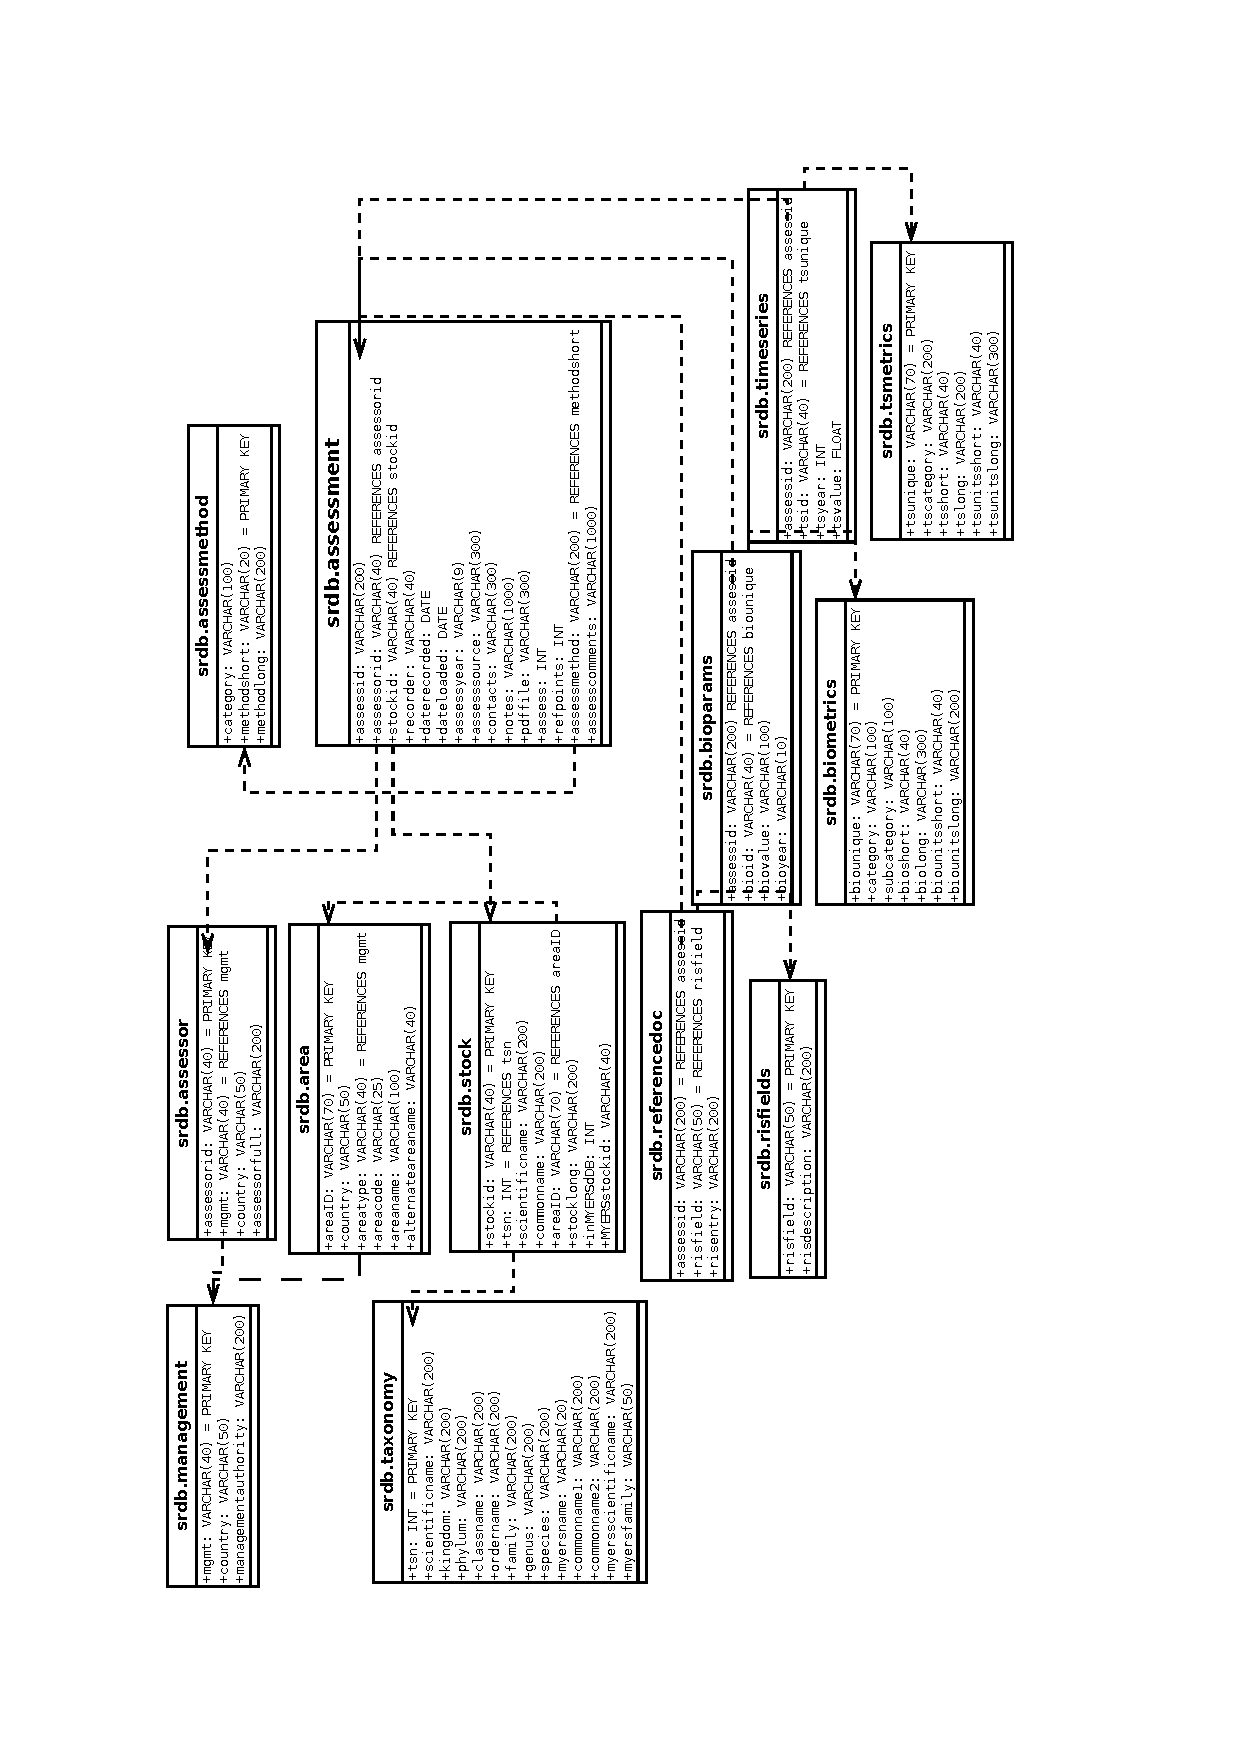
\includegraphics[width=15cm]{/home/srdbadmin/SQLpg/srdb/trunk/doc/srdb-ERD.pdf}
\end{center}
\caption{Entity relationship diagram of the RAM legacy database.}\label{fig:ERD}
\end{figure}

%%% latex table generated in R 2.9.1 by xtable 1.5-6 package
% Wed Jul 28 15:08:19 2010
\begin{longtable}{p{1.8cm}p{3.5cm}p{3.5cm}p{3cm}cccp{0.9cm}cp{0.9cm}c}
  \hline
mgmt & stock & scientificname & assessmethod & timespan & currentyear & Bratio & bfromassessment & Uratio & ufromassessment & ref \\ 
  \hline
AFMA & Bight redfish Southeast Australia & \textit{Centroberyx gerrardi} & Integrated Analysis & 1958-2007 &  &  &  &  &  & \cite{BIGHTREDDEEPFLATSE.pdf} \\ 
  AFMA & New Zealand ling Eastern half of Southeast Australia & \textit{Genypterus blacodes} & Integrated Analysis & 1968-2007 & 2007 & 0.59 & yes & 2.20 & no & \cite{NZLINGSE.pdf} \\ 
  AFMA & New Zealand ling Western half of Southeast Australia & \textit{Genypterus blacodes} & Integrated Analysis & 1968-2007 &  &  &  &  &  & \cite{NZLINGSE.pdf} \\ 
  AFMA & Orange roughy Cascade Plateau & \textit{Hoplostethus atlanticus} & Integrated Analysis & 1987-2006 & 2006 & 1.76 & no & 0.34 & no & \cite{CSIRO-Cascade-Plateau-Stock-Assessment-2006.pdf} \\ 
  AFMA & Orange roughy Southeast Australia & \textit{Hoplostethus atlanticus} & Integrated Analysis & 1978-2007 & 2007 & 0.52 & yes & 0.29 & no & \cite{OROUGHYSE.pdf} \\ 
  AFMA & Jackass morwong Southeast Australia & \textit{Nemadactylus macropterus} & Integrated Analysis & 1913-2007 & 2007 & 0.31 & yes & 1.80 & no & \cite{MORWONGSE.pdf} \\ 
  AFMA & Tiger flathead Southeast Australia & \textit{Neoplatycephalus richardsoni} & Integrated Analysis & 1913-2006 & 2006 & 1.99 & yes & 1.03 & no & \cite{TIGERFLATSE.pdf} \\ 
  AFMA & Northern Australia brown tiger shrimp & \textit{Penaeus esculentus} & Biomass dynamics model & 1970-2006 &  &  &  &  &  & \cite{NORTHPRAWNS.pdf} \\ 
  AFMA & Northern Australia grooved Tiger Prawn & \textit{Penaeus esculentus} & Biomass dynamics model & 1970-2006 &  &  &  &  &  & \cite{NORTHPRAWNS.pdf} \\ 
  AFMA & Deepwater flathead Southeast Australia & \textit{Platycephalus conatus} & Integrated Analysis & 1978-2007 & 2007 & 1.51 & yes & 0.61 & no & \cite{BIGHTREDDEEPFLATSE.pdf} \\ 
  AFMA & Tasmanian giant crab Tasmania & \textit{Pseudocarcinus gigas} & Unknown & 1990-2007 & 2007 & 0.50 & no & 1.71 & no & \cite{JENSEN_TASGIANTCRAB_2008.pdf} \\ 
  AFMA & common gemfish Southeast Australia & \textit{Rexea solandri} & Integrated Analysis & 1966-2007 & 2007 & 0.25 & yes & 0.39 & no & \cite{GEMFISHSE.pdf} \\ 
  AFMA & Blue Warehou Eastern half of Southeast Australia & \textit{Seriolella brama} & Integrated Analysis & 1984-2006 & 2006 & 0.49 & yes & 0.84 & no & \cite{WAREHOUSE.pdf} \\ 
  AFMA & Blue Warehou Western half of Southeast Australia & \textit{Seriolella brama} & Integrated Analysis & 1984-2006 & 2006 & 0.41 & yes & 2.04 & no & \cite{WAREHOUSE.pdf} \\ 
  AFMA & Silverfish Southeast Australia & \textit{Seriolella punctata} & Integrated Analysis & 1978-2006 & 2006 & 1.03 & yes & 0.79 & no & \cite{SILVERFISHSE.pdf} \\ 
  AFMA & School whiting Southeast Australia & \textit{Sillago flindersi} & Integrated Analysis & 1945-2007 & 2007 & 0.66 & yes & 0.82 & no & \cite{SWHITSE.pdf} \\ 
  CCAMLR & Antarctic toothfish Ross Sea & \textit{Dissostichus mawsoni} & Integrated Analysis & 1995-2007 & 2007 & 1.76 & no & 0.32 & yes & \cite{ATOOTHFISHRS.pdf} \\ 
  CFP & Argentine anchoita Northern Argentina & \textit{Engraulis anchoita} & VPA & 1989-2007 & 2007 & 1.37 & yes & 0.17 & yes & \cite{Hansen-ANCHOVY-N-2007.pdf} \\ 
  CFP & Argentine anchoita Southern Argentina & \textit{Engraulis anchoita} & Biomass dynamics model & 1992-2007 & 2007 & 3.13 & yes & 0.04 & yes & \cite{Hansen-ANCHOVY-S-2007.pdf} \\ 
  CFP & Patagonian grenadier Southern Argentina & \textit{Macruronus magellanicus} & VPA & 1983-2006 & 2006 & 1.82 & yes & 0.60 & yes & \cite{Giussi-hoki-2007.pdf} \\ 
  CFP & Argentine hake Northern Argentina & \textit{Merluccius hubbsi} & VPA & 1985-2007 & 2007 & 0.16 & yes & 1.26 & yes & \cite{Irusta-hake-N-2007.pdf} \\ 
  CFP & Argentine hake Southern Argentina & \textit{Merluccius hubbsi} & VPA & 1985-2008 & 2008 & 0.34 & yes & 1.49 & yes & \cite{Renzi-hake-S-2009.pdf} \\ 
  CFP &  Southern blue whiting Southern Argentina & \textit{Micromesistius australis} & VPA & 1985-2007 &  &  &  &  &  & \cite{Giussi-polaca-2007.pdf} \\ 
  DETMCM & Patagonian toothfish South Africa Subantarctic Prince Edward Islands & \textit{Dissostichus eleginoides} & Biomass dynamics model & 1960-2008 &  &  &  &  &  & \cite{Branch-SA-Toothfish-2007.pdf} \\ 
  DETMCM & Anchovy South Africa & \textit{Engraulis encrasicolus} & Statistical catch at age model & 1984-2006 & 2006 & 0.97 & no & 0.36 & no & \cite{ANCHOSA.pdf} \\ 
  DETMCM & Kingklip South Africa & \textit{Genypterus capensis} & Biomass dynamics model & 1932-2008 & 2008 & 1.20 & yes & 0.55 & no & \cite{Branch-SA-Kingklip-2008.pdf} \\ 
  DETMCM & South African abalone South Africa & \textit{Haliotis midae} & Statistical catch at age model & 1951-2008 &  &  &  &  &  & \cite{Plaganyi-SA-abalone-2008NOVSWG-AB21.pdf} \\ 
  DETMCM & South African west coast rock lobster South Africa Areas 1-2 & \textit{Jasus lalandii} & Statistical catch at age model & 1910-2008 &  &  &  &  &  & \cite{Johnston-SAWestRockLobster-2007.pdf} \\ 
  DETMCM & South African west coast rock lobster South Africa Areas 3-4 & \textit{Jasus lalandii} & Statistical catch at age model & 1910-2008 &  &  &  &  &  & \cite{Johnston-SAWestRockLobster-2007.pdf} \\ 
  DETMCM & South African west coast rock lobster South Africa Areas 5-6 & \textit{Jasus lalandii} & Statistical catch at age model & 1910-2008 &  &  &  &  &  & \cite{Johnston-SAWestRockLobster-2007.pdf} \\ 
  DETMCM & South African west coast rock lobster South Africa Area 7 & \textit{Jasus lalandii} & Statistical catch at age model & 1910-2008 &  &  &  &  &  & \cite{Johnston-SAWestRockLobster-2007.pdf} \\ 
  DETMCM & South African west coast rock lobster South Africa Area 8 & \textit{Jasus lalandii} & Statistical catch at age model & 1910-2008 &  &  &  &  &  & \cite{Johnston-SAWestRockLobster-2007.pdf} \\ 
  DETMCM & Shallow-water cape hake South Africa & \textit{Merluccius capensis} & Biomass dynamics model & 1917-2008 & 2008 & 2.30 & yes & 0.40 & no & \cite{SA-Mparadoxus-2008-IWS-DEC08-H-5.pdf} \\ 
  DETMCM & Deep-water cape hake South Africa & \textit{Merluccius paradoxus} & Biomass dynamics model & 1917-2008 &  &  &  &  &  & \cite{SA-Mparadoxus-2008-IWS-DEC08-H-5.pdf} \\ 
  DETMCM & Southern spiny lobster South Africa South coast & \textit{Palinurus gilchristi} & Statistical catch at age model & 1973-2008 & 2008 & 0.51 & no & 1.50 & no & \cite{Johnston-SASouthRockLobster-2008.pdf} \\ 
  DETMCM & Sardine South Africa & \textit{Sardinops sagax} & Statistical catch at age model & 1984-2006 & 2006 & 0.75 & no & 0.55 & no & \cite{deMoorSASardineAssessment-Sep07.pdf} \\ 
  DETMCM & Cape horse mackerel South Africa South coast & \textit{Trachurus capensis} & Biomass dynamics model & 1950-2007 & 2007 & 1.47 & no & 0.76 & no & \cite{Johnston-SAHorseMackerel-2007.pdf} \\ 
  DFO & Herring Scotian Shelf and Bay of Fundy & \textit{Clupea harengus} & VPA & 1965-2006 &  &  &  &  &  & \cite{NAFO-HERR4VWX-2006.pdf} \\ 
  DFO & Herring NAFO 4R fall spawners & \textit{Clupea harengus} & VPA & 1971-2003 &  &  &  &  &  & \cite{NAFO-HERR4RSP-2004.pdf} \\ 
  DFO & Herring NAFO 4R spring spawners & \textit{Clupea harengus} & VPA & 1963-2004 &  &  &  &  &  & \cite{NAFO-HERR4RSP-2004.pdf} \\ 
  DFO & Herring NAFO 4T fall spawners & \textit{Clupea harengus} & VPA & 1974-2007 &  &  &  &  &  & \cite{NAFO-HERR4TFA-2007.pdf} \\ 
  DFO & Herring NAFO 4T spring spawners & \textit{Clupea harengus} & VPA & 1974-2007 &  &  &  &  &  & \cite{NAFO-HERR4TFA-2007.pdf} \\ 
  DFO & Pacific herring Central Coast & \textit{Clupea pallasii} & Statistical catch at age model & 1951-2007 & 2007 & 0.30 & no & 0.11 & no & \cite{RES2007_002_e.pdf} \\ 
  DFO & Pacific herring Prince Rupert District & \textit{Clupea pallasii} & Statistical catch at age model & 1951-2007 & 2007 & 0.16 & no & 0.32 & no & \cite{RES2007_002_e.pdf} \\ 
  DFO & Pacific herring Queen Charlotte Islands & \textit{Clupea pallasii} & Statistical catch at age model & 1951-2007 & 2007 & 0.20 & no & 0.00 & no & \cite{RES2007_002_e.pdf} \\ 
  DFO & Pacific herring Straight of Georgia & \textit{Clupea pallasii} & Statistical catch at age model & 1951-2007 & 2007 & 0.91 & no & 0.40 & no & \cite{RES2007_002_e.pdf} \\ 
  DFO & Pacific herring West Coast of Vancouver Island & \textit{Clupea pallasii} & Statistical catch at age model & 1951-2007 & 2007 & 0.03 & no & 0.00 & no & \cite{RES2007_002_e.pdf} \\ 
  DFO & Pacific cod Hecate Strait & \textit{Gadus macrocephalus} & Biomass dynamics model & 1956-2005 & 2004 & 0.37 & no & 0.25 & no & \cite{RES2005_026_Cod.pdf} \\ 
  DFO & Pacific cod West Coast of Vancouver Island & \textit{Gadus macrocephalus} & Biomass dynamics model & 1956-2002 & 2001 & 0.28 & no & 0.61 & no & \cite{ref2002-113.pdf} \\ 
  DFO & Atlantic cod NAFO 5Zjm & \textit{Gadus morhua} & VPA & 1978-2003 & 2002 & 0.34 & no & 0.45 & no & \cite{NAFO-COD5Zjm-2003.pdf} \\ 
  DFO & Atlantic cod NAFO 2J3KL inshore & \textit{Gadus morhua} & VPA & 1959-2006 & 2005 & 1.60 & no & 0.14 & no & \cite{DFO-COD2J3KLIS-2006.pdf} \\ 
  DFO & Atlantic cod NAFO 3Ps & \textit{Gadus morhua} & VPA & 1959-2004 & 2004 & 0.49 & no & 0.41 & no & \cite{DFO-COD3Ps-2004.pdf} \\ 
  DFO & Atlantic cod NAFO 3Pn4RS & \textit{Gadus morhua} & VPA & 1964-2007 & 2006 & 0.09 & no & 0.79 & no & \cite{DFO-COD3Pn4Rs-2007.pdf} \\ 
  DFO & Atlantic cod NAFO 4TVn & \textit{Gadus morhua} & VPA & 1965-2007 & 2006 & 0.17 & no & 0.32 & no & \cite{NAFO-COD4TVn-2007.pdf} \\ 
  DFO & Rock sole Hecate Strait & \textit{Lepidopsetta bilineata} & Statistical catch at age model & 1945-2001 & 2001 & 1.03 & no & 0.45 & no & \cite{Flat99.pdf} \\ 
  DFO & Haddock NAFO-4X5Y & \textit{Melanogrammus aeglefinus} & VPA & 1960-2003 & 2003 & 0.85 & no & 0.33 & no & \cite{NAFO-HAD4X5Y-2003.pdf} \\ 
  DFO & Haddock NAFO-5Zejm & \textit{Melanogrammus aeglefinus} & VPA & 1968-2003 & 2002 & 1.00 & no & 0.65 & no & \cite{NAFO-HAD5Zejm-2003.pdf} \\ 
  DFO & English sole Hecate Strait & \textit{Parophrys vetulus} & Statistical catch at age model & 1944-2001 & 2001 & 1.23 & no & 0.37 & no & \cite{Flat99.pdf} \\ 
  DFO & Pollock NAFO-4VWX5Zc & \textit{Pollachius virens} & VPA & 1974-2007 & 2006 & 0.56 & no & 0.30 & no & \cite{NAFO-POLL4VWX5Zc-2006.pdf} \\ 
  IATTC & Yellowfin tuna Eastern Pacific & \textit{Thunnus albacares} & Statistical catch at age model & 1975-2007 &  &  &  &  &  & \cite{SAR8-YFT-ENG.pdf} \\ 
  IATTC & Bigeye tuna Eastern Pacific & \textit{Thunnus obesus} & Integrated Analysis & 1975-2007 &  &  &  &  &  & \cite{JENSEN_BETEPAC_2008.pdf} \\ 
  ICCAT & Skipjack tuna Eastern Atlantic & \textit{Katsuwonus pelamis} & Biomass dynamics model & 1950-2006 & 2006 & 1.71 & no & 0.27 & yes & \cite{JENSEN-YFINATL-2008.pdf} \\ 
  ICCAT & Skipjack tuna Western Atlantic & \textit{Katsuwonus pelamis} & Biomass dynamics model & 1952-2006 & 2006 & 1.72 & no & 0.32 & yes & \cite{JENSEN-YFINATL-2008.pdf} \\ 
  ICCAT & Albacore tuna North Atlantic & \textit{Thunnus alalunga} & VPA & 1929-2005 & 2005 & 0.81 & yes & 1.49 & yes & \cite{ref2007-ALB-STOCK-ASSESS-REP.pdf} \\ 
  ICCAT & Yellowfin tuna Atlantic & \textit{Thunnus albacares} & VPA & 1970-2006 & 2006 & 1.07 & yes & 0.81 & yes & \cite{JENSEN-YFINATL-2008.pdf} \\ 
  ICCAT & Bigeye tuna Atlantic & \textit{Thunnus obesus} & Biomass dynamics model & 1950-2005 & 2005 & 0.90 & no & 0.87 & yes & \cite{JENSEN-BIGEYEATL-2008.pdf} \\ 
  ICCAT & Bluefin tuna Eastern Atlantic & \textit{Thunnus thynnus} & VPA & 1969-2007 & 2007 & 0.34 & yes & 9.38 & yes & \cite{ref2008-BFT-STOCK-ASSESS-REP.pdf} \\ 
  ICCAT & Bluefin tuna Western Atlantic & \textit{Thunnus thynnus} & VPA & 1969-2007 & 2007 & 0.57 & yes & 1.33 & yes & \cite{ref2008-BFT-STOCK-ASSESS-REP.pdf} \\ 
  ICCAT & Swordfish Mediterranean Sea & \textit{Xiphias gladius} & Biomass dynamics model & 1968-2006 & 2006 & 0.94 & yes & 1.27 & yes & \cite{ICCAT-Mediterranean-Xiphiasgladius-2007.pdf} \\ 
  ICCAT & Swordfish North Atlantic & \textit{Xiphias gladius} & Biomass dynamics model & 1978-2007 & 2005 & 0.99 & yes & 0.88 & yes & \cite{JENSEN-SWORDSATL-2007.pdf} \\ 
  ICCAT & Swordfish South Atlantic & \textit{Xiphias gladius} & Biomass dynamics model & 1970-2005 & 2005 & 1.54 & yes & 0.49 & yes & \cite{JENSEN-SWORDSATL-2007.pdf} \\ 
  ICES & Sandeel North Sea & \textit{Ammodytes marinus} & VPA & 1983-2007 & 2007 & 0.92 & no & 0.24 & no & \cite{ICES-WGNSSK-2007.pdf} \\ 
  ICES & Herring ICES 22-24-IIIa & \textit{Clupea harengus} & Statistical catch at age model & 1991-2006 & 2006 & 0.73 & no & 1.02 & no & \cite{ICES-HAWG-2007.pdf} \\ 
  ICES & Herring Northern Irish Sea & \textit{Clupea harengus} & Statistical catch at age model & 1960-2006 & 2006 & 0.72 & no & 0.34 & no & \cite{ICES-HAWG-2007.pdf} \\ 
  ICES & Herring North Sea & \textit{Clupea harengus} & Statistical catch at age model & 1960-2007 & 2006 & 0.65 & no & 1.32 & no & \cite{ICES-HAWG-2007.pdf} \\ 
  ICES & Herring ICES VIa & \textit{Clupea harengus} & Statistical catch at age model & 1957-2006 & 2006 & 0.18 & no & 1.59 & no & \cite{ICES-HAWG-2007.pdf} \\ 
  ICES & Herring ICES VIa-VIIb-VIIc & \textit{Clupea harengus} & VPA & 1969-2000 & 2000 & 0.50 & no & 1.04 & no & \cite{ICES-HAWG-2007.pdf} \\ 
  ICES & Herring ICES 25-32 & \textit{Clupea harengus} & VPA & 1973-2006 & 2006 & 0.69 & no & 0.79 & no & \cite{ICES-WGBFAS-2007.pdf} \\ 
  ICES & Herring ICES 30 & \textit{Clupea harengus} & VPA & 1972-2007 & 2006 & 1.19 & no & 1.10 & no & \cite{ICES-WGBFAS-2007.pdf} \\ 
  ICES & Herring ICES 31 & \textit{Clupea harengus} & VPA & 1979-2006 & 2006 & 0.29 & no & 1.60 & no & \cite{ICES-WGBFAS-2007.pdf} \\ 
  ICES & Herring Iceland (Summer spawners) & \textit{Clupea harengus} & VPA & 1983-2007 & 2006 & 1.00 & no & 0.79 & no & \cite{ICES-NWWG-2007.pdf} \\ 
  ICES & Herring ICES 28 & \textit{Clupea harengus} & VPA & 1976-2007 & 2006 & 1.21 & no & 0.87 & no & \cite{ICES-WGBFAS-2007.pdf} \\ 
  ICES & Anchovy ICES VIII & \textit{Engraulis encrasicolus} & Biomass dynamics model & 1986-2007 &  &  &  &  &  & \cite{ICES-WGMHSA007.pdf} \\ 
  ICES & Atlantic cod coastal Norway & \textit{Gadus morhua} & VPA & 1982-2006 & 2006 & 0.27 & no & 2.17 & no & \cite{ICES-AFWG-2007.pdf} \\ 
  ICES & Atlantic cod Northeast Arctic & \textit{Gadus morhua} & VPA & 1943-2006 & 2006 & 0.56 & no & 1.42 & no & \cite{ICES-AFWG-2007.pdf} \\ 
  ICES & Atlantic cod Faroe Plateau & \textit{Gadus morhua} & VPA & 1959-2006 & 2006 & 0.26 & no & 1.52 & no & \cite{ICES-NWWG-2007.pdf} \\ 
  ICES & Atlantic cod Iceland & \textit{Gadus morhua} & Statistical catch at age model & 1952-2006 & 2006 & 0.46 & no & 1.17 & no & \cite{ICES-NWWG-2007.pdf} \\ 
  ICES & Atlantic cod Baltic Areas 22 and 24 & \textit{Gadus morhua} & VPA & 1969-2007 & 2006 & 0.36 & no & 1.43 & no & \cite{ICES-WGBFAS-2007.pdf} \\ 
  ICES & Atlantic cod Baltic Areas 25-32 & \textit{Gadus morhua} & VPA & 1964-2007 & 2006 & 0.16 & no & 1.46 & no & \cite{ICES-WGBFAS-2007.pdf} \\ 
  ICES & Atlantic cod Kattegat & \textit{Gadus morhua} & VPA & 1970-2006 & 2006 & 0.19 & no & 0.31 & no & \cite{ICES-WGBFAS-2007.pdf} \\ 
  ICES & Atlantic cod Irish Sea & \textit{Gadus morhua} & VPA & 1968-2006 & 2006 & 0.15 & no & 0.56 & no & \cite{ICES-WGNSDS-2007.pdf} \\ 
  ICES & Atlantic cod West of Scotland & \textit{Gadus morhua} & Statistical catch at age model & 1977-2006 & 2006 & 0.12 & no & 0.42 & no & \cite{ICES-WGNSDS-2007.pdf} \\ 
  ICES & Atlantic cod North Sea & \textit{Gadus morhua} & VPA & 1962-2007 & 2006 & 0.19 & no & 0.80 & no & \cite{ICES-WGNSSK-2007.pdf} \\ 
  ICES & Fourspotted megrim ICES VIIIc-IXa & \textit{Lepidorhombus boscii} & VPA & 1986-2006 & 2006 & 0.70 & no & 1.01 & no & \cite{ICES-WGHMM-2007.pdf} \\ 
  ICES & Megrim ICES VIIIc-IXa & \textit{Lepidorhombus whiffiagonis} & VPA & 1985-2007 & 2006 & 0.43 & no & 1.07 & no & \cite{ICES-WGHMM-2007.pdf} \\ 
  ICES & Capelin Barents Sea & \textit{Mallotus villosus} & Unknown & 1965-2007 & 2006 & 0.17 & no & 0.00 & no & \cite{ICES-AFWG-2007.pdf} \\ 
  ICES & Capelin Iceland & \textit{Mallotus villosus} & Survey index & 1977-2007 & 2006 & 0.49 & no & 0.85 & no & \cite{ICES-NWWG-2007.pdf} \\ 
  ICES & Haddock Northeast Arctic & \textit{Melanogrammus aeglefinus} & VPA & 1947-2006 & 2006 & 1.10 & no & 1.06 & no & \cite{ICES-AFWG-2007.pdf} \\ 
  ICES & Haddock Faroe Plateau & \textit{Melanogrammus aeglefinus} & VPA & 1955-2006 & 2006 & 0.85 & no & 1.07 & no & \cite{ICES-NWWG-2007.pdf} \\ 
  ICES & Haddock Iceland & \textit{Melanogrammus aeglefinus} & VPA & 1977-2007 & 2007 & 0.98 & no & 1.23 & no & \cite{ICES-NWWG-2007.pdf} \\ 
  ICES & Haddock Irish Sea & \textit{Melanogrammus aeglefinus} & Survey index & 1972-2006 &  &  &  &  &  & \cite{ICES-WGNSDS-2007.pdf} \\ 
  ICES & Haddock West of Scotland & \textit{Melanogrammus aeglefinus} & Statistical catch at age model & 1977-2006 & 2006 & 0.58 & no & 0.73 & no & \cite{ICES-WGNSDS-2007.pdf} \\ 
  ICES & Haddock ICES IIIa and North Sea & \textit{Melanogrammus aeglefinus} & VPA & 1963-2006 & 2006 & 0.62 & no & 0.25 & no & \cite{ICES-WGNSSK-2007.pdf} \\ 
  ICES & Haddock Rockall Bank & \textit{Melanogrammus aeglefinus} & VPA & 1990-2007 & 2006 & 1.10 & no & 0.52 & no & \cite{ICES-WGNSDS-2007.pdf} \\ 
  ICES & Haddock ICES VIIb-k & \textit{Melanogrammus aeglefinus} & VPA & 1993-2006 & 2006 & 1.37 & no & 0.41 & no & \cite{ICES-WGSSDS-2007.pdf} \\ 
  ICES & Whiting ICES VIa & \textit{Merlangius merlangus} & Survey index & 1984-2007 &  &  &  &  &  & \cite{ICES-WGNSDS-2007.pdf} \\ 
  ICES & Whiting ICES IIIa, VIId and North Sea & \textit{Merlangius merlangus} & VPA & 1979-2006 & 2006 & 0.33 & no & 1.04 & no & \cite{ICES-WGNSSK-2007.pdf} \\ 
  ICES & Whiting ICES VIIe-k & \textit{Merlangius merlangus} & VPA & 1982-2007 & 2006 & 0.44 & no & 1.25 & no & \cite{ICES-WGSSDS-2007.pdf} \\ 
  ICES & Hake Northeast Atlantic North & \textit{Merluccius merluccius} & VPA & 1977-2007 & 2006 & 1.04 & no & 0.74 & no & \cite{ICES-WGHMM-2007.pdf} \\ 
  ICES & Hake Northeast Atlantic South & \textit{Merluccius merluccius} & VPA & 1982-2007 &  &  &  &  &  & \cite{ICES-WGHMM-2007.pdf} \\ 
  ICES & Whiting Northeast Atlantic & \textit{Micromesistius poutassou} & Integrated Analysis & 1980-2007 & 2006 & 0.67 & no & 1.66 & no & \cite{ICES-WGNPBW-2007.pdf} \\ 
  ICES & European Plaice Irish Sea & \textit{Pleuronectes platessa} & Statistical catch at age model & 1962-2006 & 2006 & 1.07 & no & 0.23 & no & \cite{ICES-WGNSDS-2007.pdf} \\ 
  ICES & European Plaice ICES VIId & \textit{Pleuronectes platessa} & VPA & 1979-2006 &  &  &  &  &  & \cite{ICES-WGNSSK-2007.pdf} \\ 
  ICES & European Plaice ICES IIIa & \textit{Pleuronectes platessa} & VPA & 1976-2006 &  &  &  &  &  & \cite{ICES-WGNSSK-2007.pdf} \\ 
  ICES & European Plaice North Sea & \textit{Pleuronectes platessa} & VPA & 1956-2006 &  &  &  &  &  & \cite{ICES-WGNSSK-2007.pdf} \\ 
  ICES & European Plaice ICES VIIf-g & \textit{Pleuronectes platessa} & VPA & 1976-2006 & 2006 & 0.65 & no & 0.41 & no & \cite{ICES-WGSSDS-2007.pdf} \\ 
  ICES & European Plaice ICES VIIe & \textit{Pleuronectes platessa} & VPA & 1975-2006 & 2006 & 0.51 & no & 1.39 & no & \cite{ICES-WGSSDS-2007.pdf} \\ 
  ICES & Pollock Northeast Arctic & \textit{Pollachius virens} & VPA & 1957-2006 & 2006 & 1.70 & no & 0.60 & no & \cite{ICES-AFWG-2007.pdf} \\ 
  ICES & Pollock Faroe Plateau & \textit{Pollachius virens} & VPA & 1958-2006 & 2006 & 0.99 & no & 1.52 & no & \cite{ICES-NWWG-2007.pdf} \\ 
  ICES & Pollock ICES IIIa, VI and North Sea & \textit{Pollachius virens} & VPA & 1964-2006 & 2006 & 0.57 & no & 0.97 & no & \cite{ICES-WGNSSK-2007.pdf} \\ 
  ICES & Greenland halibut Northeast Arctic & \textit{Reinhardtius hippoglossoides} & VPA & 1959-2007 & 2006 & 0.36 & no & 1.20 & no & \cite{ICES-AFWG-2007.pdf} \\ 
  ICES & European pilchard ICES VIIIc-IXa & \textit{Sardina pilchardus} & Statistical catch at age model & 1978-2007 &  &  &  &  &  & \cite{ICES-WGMHSA07.pdf} \\ 
  ICES & Mackerel ICES Northeast Atlantic & \textit{Scomber scombrus} & Statistical catch at age model & 1972-2007 & 2006 & 0.98 & no & 0.73 & no & \cite{ICES-WGMHSA07.pdf} \\ 
  ICES & Golden Redfish Northeast Arctic & \textit{Sebastes norvegicus} & Statistical catch at age model & 1986-2006 & 2006 & 0.29 & no & 2.65 & no & \cite{ICES-AFWG-2007.pdf} \\ 
  ICES & common European sole ICES Kattegat and Skagerrak & \textit{Solea vulgaris} & VPA & 1982-2007 & 2006 & 1.25 & no & 0.54 & no & \cite{ICES-WGBFAS-2007.pdf} \\ 
  ICES & common European sole Bay of Biscay & \textit{Solea vulgaris} & VPA & 1982-2006 & 2006 & 0.76 & no & 1.00 & no & \cite{ICES-WGHMM-2007.pdf} \\ 
  ICES & common European sole Irish Sea & \textit{Solea vulgaris} & VPA & 1968-2006 & 2006 & 0.36 & no & 1.16 & no & \cite{ICES-WGNSDS-2007.pdf} \\ 
  ICES & common European sole North Sea & \textit{Solea vulgaris} & VPA & 1956-2006 &  &  &  &  &  & \cite{ICES-WGNSSK-2007.pdf} \\ 
  ICES & common European sole ICES VIId & \textit{Solea vulgaris} & VPA & 1981-2006 &  &  &  &  &  & \cite{ICES-WGNSSK-2007.pdf} \\ 
  ICES & common European sole Celtic Sea & \textit{Solea vulgaris} & VPA & 1970-2006 & 2006 & 0.90 & no & 0.95 & no & \cite{ICES-WGSSDS-2007.pdf} \\ 
  ICES & common European sole Western English Channel & \textit{Solea vulgaris} & VPA & 1968-2006 & 2006 & 0.51 & no & 1.74 & no & \cite{ICES-WGSSDS-2007.pdf} \\ 
  ICES & Sprat North Sea & \textit{Sprattus sprattus} & Statistical catch at age model & 1995-2007 &  &  &  &  &  & \cite{ICES-HAWG-2007.pdf} \\ 
  ICES & Sprat ICES Baltic Areas 22-32 & \textit{Sprattus sprattus} & VPA & 1973-2007 & 2006 & 1.13 & no & 1.27 & no & \cite{ICES-WGBFAS-2007.pdf} \\ 
  ICES & Norway pout North Sea & \textit{Trisopterus esmarkii} & VPA & 1983-2007 & 2006 & 0.90 & no & 0.33 & no & \cite{ICES-WGNSSK-2007.pdf} \\ 
  IMARPE & Peruvian anchoveta North-Central Peru & \textit{Engraulis ringens} & VPA & 1963-2004 &  &  &  &  &  & \cite{Cahuin_etal_2009.pdf} \\ 
  IOTC & Bigeye tuna Indian Ocean & \textit{Thunnus obesus} & Biomass dynamics model & 1957-2006 & 2004 & 1.23 & yes & 0.97 & yes & \cite{JENSEN-BIGEYEIO-2007.pdf} \\ 
  IPHC & Pacific halibut North Pacific & \textit{Hippoglossus stenolepis} & Statistical catch at age model & 1988-2009 & 2008 & 0.54 & no & 2.01 & no & \cite{hare-clark08.pdf} \\ 
  MFish & Black oreo West end of Chatham Rise & \textit{Allocyttus niger} & Integrated Analysis & 1973-2007 & 2007 & 0.99 & yes & 0.82 & yes & \cite{CORDUEperscomm.pdf} \\ 
  MFish & Australian salmon New Zealand & \textit{Arripis trutta} & Integrated Analysis & 1975-2006 & 2006 & 1.64 & yes & 0.33 & yes & \cite{CORDUEperscomm.pdf} \\ 
  MFish & New Zealand snapper New Zealand Area 8 & \textit{Chrysophrys auratus} & Integrated Analysis & 1931-2005 & 2005 & 0.35 & yes & 2.50 & yes & \cite{CORDUEperscomm.pdf} \\ 
  MFish & New Zealand ling New Zealand Areas LIN 3 and 4 & \textit{Genypterus blacodes} & Integrated Analysis & 1972-2007 & 2007 & 3.07 & yes & 0.09 & yes & \cite{CORDUEperscomm.pdf} \\ 
  MFish & New Zealand ling New Zealand Areas LIN 5 and 6 & \textit{Genypterus blacodes} & Integrated Analysis & 1972-2007 & 2007 & 3.96 & yes & 0.10 & yes & \cite{CORDUEperscomm.pdf} \\ 
  MFish & New Zealand ling New Zealand Area LIN 6b & \textit{Genypterus blacodes} & Integrated Analysis & 1980-2006 & 2006 & 2.19 & yes & 0.11 & yes & \cite{CORDUEperscomm.pdf} \\ 
  MFish & New Zealand ling New Zealand Area LIN 72 & \textit{Genypterus blacodes} & Integrated Analysis & 1972-2007 & 2007 & 2.49 & yes & 0.32 & yes & \cite{CORDUEperscomm.pdf} \\ 
  MFish & New Zealand ling New Zealand Area LIN 7WC - WCSI & \textit{Genypterus blacodes} & Integrated Analysis & 1972-2008 & 2008 & 2.21 & yes & 0.13 & yes & \cite{CORDUEperscomm.pdf} \\ 
  MFish & New Zealand abalone species New Zealand Area PAU 5A & \textit{Haliotis iris} & Integrated Analysis & 1964-2006 & 2006 & 0.72 & no & 2.83 & no & \cite{ref07-09-FAR.pdf} \\ 
  MFish & New Zealand abalone species New Zealand Area PAU 5B & \textit{Haliotis iris} & Integrated Analysis & 1963-2007 & 2007 & 1.02 & no & 0.59 & no & \cite{ref08-05-FAR.pdf} \\ 
  MFish & New Zealand abalone species New Zealand Area PAU 5D & \textit{Haliotis iris} & Integrated Analysis & 1964-2006 & 2006 & 0.44 & no & 2.10 & no & \cite{ref07-09-FAR.pdf} \\ 
  MFish & New Zealand abalone species New Zealand Area PAU 7 & \textit{Haliotis iris} & Integrated Analysis & 1964-2008 & 2008 & 0.87 & no & 0.94 & no & \cite{ref09-34-FAR.pdf} \\ 
  MFish & Orange roughy New Zealand Mid East Coast & \textit{Hoplostethus atlanticus} & Integrated Analysis & 1981-2004 & 2004 & 1.20 & yes & 0.35 & yes & \cite{CORDUEperscomm.pdf} \\ 
  MFish & Red rock lobster New Zealand area CRA1 & \textit{Jasus edwardsii} & Unknown & 1945-2001 & 2001 & 1.14 & no & 0.88 & no & \cite{PALLSTARRperscomm.pdf} \\ 
  MFish & Red rock lobster New Zealand area CRA2 & \textit{Jasus edwardsii} & Unknown & 1945-2001 & 2001 & 0.53 & no & 2.12 & no & \cite{PALLSTARRperscomm.pdf} \\ 
  MFish & Red rock lobster New Zealand area CRA3 & \textit{Jasus edwardsii} & Unknown & 1945-2007 &  &  &  &  &  & \cite{PALLSTARRperscomm.pdf} \\ 
  MFish & Red rock lobster New Zealand area CRA4 & \textit{Jasus edwardsii} & Unknown & 1945-2005 & 2005 & 0.67 & no & 1.33 & no & \cite{PALLSTARRperscomm.pdf} \\ 
  MFish & Red rock lobster New Zealand area CRA5 & \textit{Jasus edwardsii} & Unknown & 1945-2002 & 2002 & 0.59 & no & 1.68 & no & \cite{PALLSTARRperscomm.pdf} \\ 
  MFish & Red rock lobster New Zealand area CRA7 & \textit{Jasus edwardsii} & Unknown & 1976-2005 & 2005 & 0.73 & no & 0.43 & no & \cite{PALLSTARRperscomm.pdf} \\ 
  MFish & Red rock lobster New Zealand area CRA8 & \textit{Jasus edwardsii} & Unknown & 1976-2005 & 2005 & 0.69 & no & 0.49 & no & \cite{PALLSTARRperscomm.pdf} \\ 
  MFish & Hoki Eastern New Zealand & \textit{Macruronus novaezelandiae} & Integrated Analysis & 1972-2007 & 2007 & 1.11 & no & 0.33 & no & \cite{FAR0804hok07.pdf} \\ 
  MFish & Hoki Western New Zealand & \textit{Macruronus novaezelandiae} & Integrated Analysis & 1972-2007 & 2007 & 0.51 & no & 0.57 & no & \cite{FAR0804hok07.pdf} \\ 
  MFish & Southern hake Chatham Rise & \textit{Merluccius australis} & Integrated Analysis & 1975-2006 & 2006 & 1.77 & yes & 0.12 & yes & \cite{CORDUEperscomm.pdf} \\ 
  MFish & Southern hake Sub-Antarctic & \textit{Merluccius australis} & Integrated Analysis & 1975-2007 & 2007 & 2.91 & yes & 0.11 & yes & \cite{CORDUEperscomm.pdf} \\ 
  MFish & Southern blue whiting Campbell Island Rise & \textit{Micromesistius australis} & Integrated Analysis & 1979-2006 & 2006 & 1.15 & yes & 0.92 & yes & \cite{CORDUEperscomm.pdf} \\ 
  MFish & Trevally New Zealand Areas TRE 7 & \textit{Pseudocaranx dentex} & Integrated Analysis & 1944-2005 & 2005 & 1.44 & yes & 0.83 & yes & \cite{CORDUEperscomm.pdf} \\ 
  MFish & Smooth oreo Chatham Rise & \textit{Pseudocyttus maculatus} & Integrated Analysis & 1979-2006 & 2006 & 2.25 & yes & 0.38 & yes & \cite{CORDUEperscomm.pdf} \\ 
  MFish & Smooth oreo West end of Chatham Rise & \textit{Pseudocyttus maculatus} & Integrated Analysis & 1973-2004 & 2004 & 1.25 & yes & 0.53 & yes & \cite{CORDUEperscomm.pdf} \\ 
  MFish & common gemfish New Zealand & \textit{Rexea solandri} & Integrated Analysis & 1952-2007 & 2006 & 1.64 & yes & 0.43 & yes & \cite{CORDUEperscomm.pdf} \\ 
  NAFO & Atlantic cod NAFO 3M & \textit{Gadus morhua} & VPA & 1959-2008 &  &  &  &  &  & \cite{NAFO-3M-COD-2008.pdf} \\ 
  NAFO & Atlantic cod NAFO 3NO & \textit{Gadus morhua} & VPA & 1953-2007 & 2006 & 0.02 & no & 0.27 & no & \cite{NAFO-3NO-COD-2007.pdf} \\ 
  NAFO & American Plaice NAFO-3LNO & \textit{Hippoglossoides platessoides} & VPA & 1955-2007 & 2006 & 0.08 & no & 0.77 & no & \cite{NAFO-GrandBanks-AmPlaice-2007.pdf} \\ 
  NAFO & American Plaice NAFO-3M & \textit{Hippoglossoides platessoides} & VPA & 1960-2007 & 2007 & 0.13 & no & 0.00 & no & \cite{NAFO-AMPL3M-2008.pdf} \\ 
  NAFO & Yellowtail Flounder NAFO 3LNO & \textit{Limanda ferruginea} & Biomass dynamics model & 1960-2009 & 2007 & 1.62 & no & 0.15 & no & \cite{NAFO-YELL3LNO-2008.pdf} \\ 
  NAFO & Redfish species NAFO 3LN & \textit{Redfish species} & Biomass dynamics model & 1959-2008 & 2008 & 1.88 & yes & 0.04 & yes & \cite{NAFO-3LN-Redfishspp-2008.pdf} \\ 
  NAFO & Redfish species NAFO 3M & \textit{Redfish species} & VPA & 1989-2006 & 2006 & 0.93 & no & 0.15 & no & \cite{NAFO-RED3M-2007.pdf} \\ 
  NAFO & Greenland halibut NAFO 23KLMNO & \textit{Reinhardtius hippoglossoides} & VPA & 1960-2006 & 2006 & 0.39 & no & 1.73 & no & \cite{NAFO-GHAL23KLMNO-2007.pdf} \\ 
  NMFS & Sablefish Eastern Bering Sea / Aleutian Islands / Gulf of Alaska & \textit{Anoplopoma fimbria} & Statistical catch at age model & 1956-2008 & 2008 & 1.05 & yes & 0.66 & yes & \cite{AFSC-SABLEFEBSAIGA-2008-Sablefish-EBS-AI-GA.pdf} \\ 
  NMFS & Sablefish Pacific Coast & \textit{Anoplopoma fimbria} & Integrated Analysis & 1900-2007 & 2007 & 0.84 & no & 0.69 & yes & \cite{NWFSC-SABLEFPCOAST-2007-Sablefish.pdf} \\ 
  NMFS & Ocean quahog Atlantic Coast & \textit{Arctica islandica} & Biomass dynamics model & 1978-2008 &  &  &  &  &  & \cite{quahog.pdf} \\ 
  NMFS & Gray triggerfish Gulf of Mexico & \textit{Balistes capriscus} & Biomass dynamics model & 1981-2004 &  &  &  &  &  & \cite{JENSEN_GTRIGGM_2006.pdf} \\ 
  NMFS & Gulf menhaden Gulf of Mexico & \textit{Brevoortia patronus} & Statistical catch at age model & 1964-2004 & 2004 & 1.08 & no & 0.48 & no & \cite{GILROY-MENHADENGM-2007.pdf} \\ 
  NMFS & Atlantic menhaden Atlantic & \textit{Brevoortia tyrannus} & Statistical catch at age model & 1940-2005 & 2005 & 0.47 & no & 0.97 & no & \cite{Atl.Menhaden-ASMFC-2006.pdf} \\ 
  NMFS & Blacknose shark Atlantic & \textit{Carcharhinus acronotus} & Biomass dynamics model & 1950-2005 &  &  &  &  &  & \cite{SmallcoastalAtl2007-SEFSC.pdf} \\ 
  NMFS & Finetooth shark Atlantic & \textit{Carcharhinus isodon} & Biomass dynamics model & 1976-2005 &  &  &  &  &  & \cite{SmallcoastalAtl2007-SEFSC.pdf} \\ 
  NMFS & Blacktip shark Atlantic & \textit{Carcharhinus limbatus} & Biomass dynamics model & 1981-2004 &  &  &  &  &  & \cite{LargeCoastalAtl2006-SEFSC.pdf} \\ 
  NMFS & Blacktip shark Gulf of Mexico & \textit{Carcharhinus limbatus} & Biomass dynamics model & 1981-2004 &  &  &  &  &  & \cite{LargeCoastalAtl2006-SEFSC.pdf} \\ 
  NMFS & Sandbar shark Atlantic & \textit{Carcharhinus plumbeus} & Biomass dynamics model & 1975-2004 &  &  &  &  &  & \cite{LargeCoastalAtl2006-SEFSC.pdf} \\ 
  NMFS & Black sea bass Mid-Atlantic Coast & \textit{Centropristis striata} & Statistical catch at age model & 1968-2007 & 2007 & 0.92 & yes & 0.67 & no & \cite{DataPoorReviewPanelReportFinal-1-20-09.pdf} \\ 
  NMFS & Snow crab Bering Sea & \textit{Chionoecetes opilio} & Biomass dynamics model & 1979-2008 & 2008 & 0.55 & yes & 1.49 & no & \cite{CRABSAFE2008.pdf} \\ 
  NMFS & Atlantic herring Northwestern Atlantic Coast & \textit{Clupea harengus} & Statistical catch at age model & 1960-2005 &  &  &  &  &  & \cite{Herring2006.pdf} \\ 
  NMFS & Pacific herring Prince William Sound & \textit{Clupea pallasii} & Statistical catch at age model & 1980-2006 &  &  &  &  &  & \cite{Hulson-etal-2008-ICESJM.pdf} \\ 
  NMFS & Pacific herring Sitka & \textit{Clupea pallasii} & Statistical catch at age model & 1978-2007 &  &  &  &  &  & \cite{Hulson-etal-2008-ICESJM.pdf} \\ 
  NMFS & Weakfish Atlantic Coast & \textit{Cynoscion regalis} & VPA & 1981-2008 &  &  &  &  &  & \cite{NEFSC-Weakfish-2009.pdf} \\ 
  NMFS & Petrale sole Northern Pacific Coast & \textit{Eopsetta jordani} & Integrated Analysis & 1910-2005 & 2005 & 1.87 & yes & 1.26 & no & \cite{ref2004-SAFE-WCpetralesole.pdf} \\ 
  NMFS & Petrale sole Southern Pacific Coast & \textit{Eopsetta jordani} & Integrated Analysis & 1874-2005 & 2005 & 1.13 & yes & 0.61 & no & \cite{ref2004-SAFE-WCpetralesole.pdf} \\ 
  NMFS & Red grouper Gulf of Mexico & \textit{Epinephelus morio} & Statistical catch at age model & 1986-2005 & 2005 & 1.27 & yes & 0.73 & yes & \cite{JENSEN-RGROUPGM-2006.pdf} \\ 
  NMFS & Snowy grouper Southern Atlantic coast & \textit{Epinephelus niveatus} & Statistical catch at age model & 1961-2002 & 2002 & 0.19 & yes & 3.08 & yes & \cite{ref2004-SEDAR-deepwatersnappergrouper.pdf} \\ 
  NMFS & Pacific cod Bering Sea and Aleutian Islands & \textit{Gadus macrocephalus} & Integrated Analysis & 1964-2008 & 2008 & 1.00 & yes & 0.93 & no & \cite{AFSC-PCODBSAI-2008-Pacific-cod-BSAI.pdf} \\ 
  NMFS & Pacific cod Gulf of Alaska & \textit{Gadus macrocephalus} & Integrated Analysis & 1964-2008 & 2008 & 0.91 & yes & 0.84 & no & \cite{AFSC-PCODGA-2008-Pacific-cod-GA.pdf} \\ 
  NMFS & Atlantic cod Georges Bank & \textit{Gadus morhua} & VPA & 1960-2008 & 2007 & 0.12 & yes & 0.72 & no & \cite{NMFS-GB-Gadusmorhua-2008.pdf} \\ 
  NMFS & Atlantic cod Gulf of Maine & \textit{Gadus morhua} & VPA & 1893-2008 & 2007 & 1.46 & no & 2.40 & yes & \cite{NMFS-GOM-Gadusmorhua-2008.pdf} \\ 
  NMFS & Witch Flounder NAFO-5Y & \textit{Glyptocephalus cynoglossus} & VPA & 1982-2008 & 2007 & 0.30 & yes & 1.45 & yes & \cite{crd0815.pdf} \\ 
  NMFS & Rex sole Gulf of Alaska & \textit{Glyptocephalus zachirus} & Statistical catch at age model & 1979-2008 &  &  &  &  &  & \cite{ref2008-SAFE-GOArex.pdf} \\ 
  NMFS & Kelp greenling Oregon Coast & \textit{Hexagrammos decagrammus} & Integrated Analysis & 1979-2005 &  &  &  &  &  & \cite{KelpGreenling_2005.pdf} \\ 
  NMFS & Flathead sole Bering Sea and Aleutian Islands & \textit{Hippoglossoides elassodon} & Statistical catch at age model & 1977-2008 & 2008 & 1.83 & yes & 0.18 & no & \cite{2008_SAFE_BSAIflathead.pdf} \\ 
  NMFS & Flathead sole Gulf of Alaska & \textit{Hippoglossoides elassodon} & Statistical catch at age model & 1978-2008 &  &  &  &  &  & \cite{2008_SAFE_GOAflathead.pdf} \\ 
  NMFS & American Plaice NAFO-5YZ & \textit{Hippoglossoides platessoides} & VPA & 1960-2008 & 2007 & 0.70 & yes & 0.30 & no & \cite{ .pdf} \\ 
  NMFS & Atlantic Halibut NAFO-5YZ & \textit{Hippoglossus hippoglossus} & Unknown & 1800-2007 &  &  &  &  &  & \cite{AtlanticHalibut5YZ2008.pdf .pdf} \\ 
  NMFS & American lobster Georges Bank & \textit{Homarus americanus} & Biomass dynamics model & 1981-2007 &  &  &  &  &  & \cite{2009-ASMFC-Am-Lob.pdf} \\ 
  NMFS & American lobster Gulf of Maine & \textit{Homarus americanus} & Biomass dynamics model & 1981-2007 &  &  &  &  &  & \cite{2009-ASMFC-Am-Lob.pdf} \\ 
  NMFS & American lobster Southern New England & \textit{Homarus americanus} & Biomass dynamics model & 1981-2007 &  &  &  &  &  & \cite{2009-ASMFC-Am-Lob.pdf} \\ 
  NMFS & Northern shortfin squid Northwestern Atlantic Coast & \textit{Illex illecebrosus} & Biomass dynamics model & 1967-2005 &  &  &  &  &  & \cite{scr06-46.pdf} \\ 
  NMFS & Northern rock sole Eastern Bering Sea and Aleutian Islands & \textit{Lepidopsetta polyxystra} & Statistical catch at age model & 1971-2008 & 2007 & 3.02 & yes & 0.21 & yes & \cite{2008_SAFE_BSAIrocksole.pdf} \\ 
  NMFS & Yellowfin sole Bering Sea and Aleutian Islands & \textit{Limanda aspera} & Statistical catch at age model & 1959-2008 & 2008 & 1.94 & yes & 0.62 & yes & \cite{AFSC-YSOLEBSAI-2008-Yellowfin sole BSAI.pdf} \\ 
  NMFS & Yellowtail flounder Cape Cod / Gulf of Maine & \textit{Limanda ferruginea} & VPA & 1935-2008 & 2007 & 0.25 & yes & 1.73 & yes & \cite{NMFS-CCGOM-Limandaferruginea-2008.pdf} \\ 
  NMFS & Yellowtail flounder Georges Bank & \textit{Limanda ferruginea} & VPA & 1935-2008 & 2007 & 0.22 & yes & 1.14 & yes & \cite{NMFS-GB-Limandaferruginea-2008.pdf} \\ 
  NMFS & Yellowtail Flounder Southern New England-Mid Atlantic & \textit{Limanda ferruginea} & VPA & 1935-2008 & 2007 & 0.13 & yes & 1.61 & yes & \cite{NMFS-SNEMATL-Limandaferruginea-2008.pdf} \\ 
  NMFS & Golden king crab Aleutian Islands Eastern segment & \textit{Lithodes aequispinus} & Statistical catch at length model & 1990-2007 &  &  &  &  &  & \cite{CRABSAFE2008.pdf} \\ 
  NMFS & Golden king crab Aleutian Islands Western segment & \textit{Lithodes aequispinus} & Statistical catch at length model & 1989-2007 &  &  &  &  &  & \cite{CRABSAFE2008.pdf} \\ 
  NMFS & Monkfish Gulf of Maine / Northern Georges Bank & \textit{Lophius americanus} & Unknown & 1964-2006 & 2006 & 1.73 & no & 0.38 & no & \cite{crd0721.pdf} \\ 
  NMFS & Monkfish Southern Georges Bank / Mid-Atlantic & \textit{Lophius americanus} & Unknown & 1964-2006 & 2006 & 1.72 & no & 0.30 & no & \cite{Monkfish2007NEFSCAssessment.pdf} \\ 
  NMFS & Tilefish Mid-Atlantic Coast & \textit{Lopholatilus chamaeleonticeps} & Biomass dynamics model & 1973-2008 & 2005 & 0.72 & no & 0.61 & no & \cite{Tilefish2005.pdf} \\ 
  NMFS & Tilefish Southern Atlantic coast & \textit{Lopholatilus chamaeleonticeps} & Statistical catch at age model & 1961-2002 & 2002 & 0.90 & yes & 1.55 & yes & \cite{2004-SEDAR-deepwatersnappergrouper.pdf} \\ 
  NMFS & Mutton snapper Southern Atlantic coast and Gulf of Mexico & \textit{Lutjanus analis} & Statistical catch at age model & 1981-2006 &  &  &  &  &  & \cite{JENSEN_MUTSNAPSATLCGM_2008.pdf} \\ 
  NMFS & Red snapper Eastern Gulf of Mexico & \textit{Lutjanus campechanus} & Statistical catch at age model & 1872-2003 &  &  &  &  &  & \cite{RedSnapper-SEDAR-2008.pdf} \\ 
  NMFS & Red snapper Southern Atlantic coast & \textit{Lutjanus campechanus} & Statistical catch at age model & 1945-2006 &  &  &  &  &  & \cite{JENSEN_RSNAPSATLC_2008.pdf} \\ 
  NMFS & Red snapper Western Gulf of Mexico & \textit{Lutjanus campechanus} & Statistical catch at age model & 1880-2003 &  &  &  &  &  & \cite{RedSnapper-SEDAR-2008.pdf} \\ 
  NMFS & Haddock NAFO-5Y & \textit{Melanogrammus aeglefinus} & VPA & 1956-2008 & 2007 & 0.99 & yes & 1.21 & no & \cite{NMFS-GOM-Melanogrammusaeglefinus-2008.pdf} \\ 
  NMFS & Haddock Georges Bank & \textit{Melanogrammus aeglefinus} & VPA & 1930-2008 &  &  &  &  &  & \cite{NMFS-5Z-Melanogrammusaeglefinus-2008.pdf} \\ 
  NMFS & Silver hake Gulf of Maine / Northern Georges Bank & \textit{Merluccius bilinearis} & Survey index & 1955-2005 &  &  &  &  &  & \cite{SilverHake-2005-NEFSC-Assessment.pdf} \\ 
  NMFS & Silver hake Southern Georges Bank / Mid-Atlantic & \textit{Merluccius bilinearis} & Survey index & 1955-2005 &  &  &  &  &  & \cite{SilverHake-2005-NEFSC-Assessment.pdf} \\ 
  NMFS & Pacific hake Pacific Coast & \textit{Merluccius productus} & Integrated Analysis & 1966-2008 & 2008 & 1.61 & yes & 0.73 & yes & \cite{NWFSC-PHAKEPCOAST-2008-Pacific-Hake-US-Canada.pdf} \\ 
  NMFS & Atlantic croaker Mid-Atlantic Coast & \textit{Micropogonias undulatus} & Biomass dynamics model & 1973-2002 & 2002 & 1.42 & yes & 0.27 & yes & \cite{2004_ASMFC_AtlCroak.pdf} \\ 
  NMFS & Dover sole Gulf of Alaska & \textit{Microstomus pacificus} & Statistical catch at age model & 1978-2010 &  &  &  &  &  & \cite{2007_SAFE_GOAdeepflat.pdf} \\ 
  NMFS & Dover sole Pacific Coast & \textit{Microstomus pacificus} & Integrated Analysis & 1910-2005 & 2005 & 1.61 & yes & 0.45 & no & \cite{2005-SAFE-WCdover.pdf} \\ 
  NMFS & Striped bass Gulf of Maine / Cape Hatteras & \textit{Morone saxatilis} & Statistical catch at age model & 1982-2006 &  &  &  &  &  & \cite{07AssessmentReport.pdf} \\ 
  NMFS & Gag Gulf of Mexico & \textit{Mycteroperca microlepis} & Unknown & 1963-2004 & 2004 & 1.00 & yes & 2.44 & yes & \cite{JENSEN_GAGGM_2007.pdf} \\ 
  NMFS & Gag Southern Atlantic coast & \textit{Mycteroperca microlepis} & Statistical catch at age model & 1962-2005 & 2005 & 0.94 & yes & 1.31 & yes & \cite{JENSEN_GAGSATLC_2006.pdf} \\ 
  NMFS & Yellowtail snapper Southern Atlantic Coast and Gulf of Mexico & \textit{Ocyurus chrysurus} & Statistical catch at age model & 1962-2001 & 2001 & 1.14 & yes & 0.61 & yes & \cite{2003_SEDAR_Yellowtailsnapper.pdf} \\ 
  NMFS & Lingcod Northern Pacific Coast & \textit{Ophiodon elongatus} & Integrated Analysis & 1956-2005 &  &  &  &  &  & \cite{2005-SAFE-WClingcod.pdf} \\ 
  NMFS & Lingcod Southern Pacific Coast & \textit{Ophiodon elongatus} & Integrated Analysis & 1956-2005 &  &  &  &  &  & \cite{2005_SAFE_Wclingcod.pdf} \\ 
  NMFS & Red porgy Southern Atlantic coast & \textit{Pagrus pagrus} & Statistical catch at age model & 1972-2004 & 2004 & 0.61 & yes & 0.39 & yes & \cite{JENSEN_RPORGYSATLC_2006.pdf} \\ 
  NMFS & Northern shrimp Gulf of Maine & \textit{Pandalus borealis} & Statistical catch at age model & 1960-2009 & 2008 & 1.58 & no & 0.56 & no & \cite{2008ShrimpAssessment.pdf} \\ 
  NMFS & Summer flounder Mid-Atlantic Coast & \textit{Paralichthys dentatus} & Statistical catch at age model & 1940-2007 &  &  &  &  &  & \cite{NMFS-MATLC-Paralichthysdentatus-2008.pdf} \\ 
  NMFS & Red king crab Bristol Bay & \textit{Paralithodes camtschaticus} & Statistical catch at length model & 1960-2008 & 2008 & 1.27 & yes & 1.05 & yes & \cite{CRABSAFE2008.pdf} \\ 
  NMFS & Red king crab Norton Sound & \textit{Paralithodes camtschaticus} & Statistical catch at length model & 1976-2008 &  &  &  &  &  & \cite{CRABSAFE2008.pdf} \\ 
  NMFS & English sole Pacific Coast & \textit{Parophrys vetulus} & Integrated Analysis & 1876-2007 & 2007 & 6.42 & yes & 0.14 & no & \cite{NWFSC-ESOLEPCOAST-2007-EnglishSole.pdf} \\ 
  NMFS & Atlantic butterfish Gulf of Maine / Cape Hatteras & \textit{Peprilus triacanthus} & Unknown & 1965-2005 &  &  &  &  &  & \cite{butterfish-assessment-2004.pdf} \\ 
  NMFS & Sea scallop Georges Bank & \textit{Placopecten magellanicus} & Statistical catch at length model & 1964-2006 & 2006 & 1.59 & no & 0.78 & no & \cite{SeaScallop2007.pdf} \\ 
  NMFS & Sea scallop Mid-Atlantic Coast & \textit{Placopecten magellanicus} & Statistical catch at length model & 1964-2006 & 2006 & 1.00 & no & 0.36 & no & \cite{SeaScallop2007.pdf} \\ 
  NMFS & Starry flounder Northern Pacific Coast & \textit{Platichthys stellatus} & Integrated Analysis & 1970-2005 & 2005 & 1.10 & yes & 0.33 & no & \cite{2005-SAFE-WCstarryflounder.pdf} \\ 
  NMFS & Starry flounder Southern Pacific Coast & \textit{Platichthys stellatus} & Integrated Analysis & 1970-2005 & 2005 & 1.55 & yes & 0.12 & no & \cite{2005-SAFE-WCstarryflounder.pdf} \\ 
  NMFS & Atka mackerel Bering Sea and Aleutian Islands & \textit{Pleurogrammus monopterygius} & Statistical catch at age model & 1976-2009 & 2009 & 1.55 & yes & 0.55 & no & \cite{2008_SAFE_BSAIatka.pdf} \\ 
  NMFS & Alaska plaice Bering Sea and Aleutian Islands & \textit{Pleuronectes quadrituberculatus} & Statistical catch at age model & 1972-2008 & 2008 & 2.46 & yes & 0.07 & yes & \cite{AFSC-ALPLAICBSAI-2008-Alaska plaice BSAI.pdf} \\ 
  NMFS & Pollock NAFO-5YZ & \textit{Pollachius virens} & Survey index & 1963-2007 &  &  &  &  &  & \cite{http://www.nefsc.noaa.gov/nefsc/publications/crd/crd0815/crd0815.pdf} \\ 
  NMFS & Bluefish Atlantic Coast & \textit{Pomatomus saltatrix} & Statistical catch at age model & 1981-2007 & 2007 & 0.81 & no & 0.79 & yes & \cite{final-2005-SAW-41-assessment.pdf} \\ 
  NMFS & Winter Flounder NAFO-5Z & \textit{Pseudopleuronectes americanus} & VPA & 1982-2007 & 2006 & 0.28 & yes & 0.25 & no & \cite{garm3k.pdf} \\ 
  NMFS & Winter Flounder NAFO-5Y & \textit{Pseudopleuronectes americanus} & Unknown & 1982-2008 &  &  &  &  &  & \cite{http://www.nefsc.noaa.gov/nefsc/publications/crd/crd0815/crd0815.pdf} \\ 
  NMFS & Winter Flounder Southern New England-Mid Atlantic & \textit{Pseudopleuronectes americanus} & VPA & 1940-2007 & 2007 & 0.09 & yes & 1.10 & no & \cite{NMFS-SNEMATL-Pseudopleuronectesamercianus-2008.pdf} \\ 
  NMFS & Longnose skate Pacific Coast & \textit{Raja rhina} & Integrated Analysis & 1915-2007 & 2007 & 1.56 & no & 0.40 & no & \cite{NWFSC-LNOSESKAPCOAST-2008-Longnose skate.pdf} \\ 
  NMFS & Greenland turbot Bering Sea and Aleutian Islands & \textit{Reinhardtius hippoglossoides} & Statistical catch at age model & 1960-2009 & 2009 & 1.48 & yes & 0.05 & yes & \cite{2008_SAFE_BSAIturbot.pdf} \\ 
  NMFS & Arrowtooth flounder Bering Sea and Aleutian Islands & \textit{Reinhardtius stomias} & Statistical catch at age model & 1970-2008 & 2008 & 2.70 & yes & 0.31 & no & \cite{AFSC-ARFLOUNDBSAI-2007-Arrowtooth flounder BSAI.pdf} \\ 
  NMFS & Arrowtooth flounder Gulf of Alaska & \textit{Reinhardtius stomias} & Statistical catch at age model & 1958-2010 & 2010 & 3.02 & yes & 0.28 & no & \cite{2008_SAFE_GOAatf.pdf} \\ 
  NMFS & Arrowtooth flounder Pacific Coast & \textit{Reinhardtius stomias} & Integrated Analysis & 1916-2007 & 2007 & 3.81 & yes & 0.21 & yes & \cite{NWFSC-ARFLOUNDPCOAST-2007-Arrowtooth flounder.pdf} \\ 
  NMFS & Atlantic sharpnose shark Atlantic & \textit{Rhizoprionodon terraenovae} & Biomass dynamics model & 1950-2005 &  &  &  &  &  & \cite{SmallcoastalAtl2007-SEFSC.pdf} \\ 
  NMFS & Vermilion snapper Gulf of Mexico & \textit{Rhomboplites aurorubens} & Biomass dynamics model & 1981-2004 &  &  &  &  &  & \cite{JENSEN_VSNAPGM_2006.pdf} \\ 
  NMFS & Vermilion snapper Southern Atlantic coast & \textit{Rhomboplites aurorubens} & Statistical catch at age model & 1946-2008 & 2007 & 0.86 & yes & 1.27 & yes & \cite{2008_SEDAR_VermillionSnapper_Satl.pdf} \\ 
  NMFS & Pacific sardine North Pacific & \textit{Sardinops sagax} & Statistical catch at age model & 1981-2008 & 2006 & 1.73 & no & 0.37 & no & \cite{2008 pac sardine.pdf} \\ 
  NMFS & Pacific sardine Pacific Coast & \textit{Sardinops sagax} & Integrated Analysis & 1981-2007 & 2006 & 1.36 & no & 0.41 & no & \cite{NOAA-TM-NMFS-SWFSC-413.pdf} \\ 
  NMFS & Pacific chub mackerel Pacific Coast & \textit{Scomber japonicus} & Statistical catch at age model & 1929-2008 &  &  &  &  &  & \cite{PFMC_2008_CPS_SAFE_App2_PMackerel.pdf} \\ 
  NMFS & King mackerel Gulf of Mexico & \textit{Scomberomorus cavalla} & VPA & 1992-2001 & 2001 & 0.93 & yes & 0.44 & no & \cite{JENSEN_KMACKGMSATLC_2004.pdf} \\ 
  NMFS & King mackerel Southern Atlantic Coast & \textit{Scomberomorus cavalla} & VPA & 1981-2001 & 2001 & 1.35 & yes & 0.56 & no & \cite{JENSEN_KMACKGMSATLC_2004.pdf} \\ 
  NMFS & Spanish mackerel Southern Atlantic Coast & \textit{Scomberomorus maculatus} & Statistical catch at age model & 1950-2008 & 2007 & 0.38 & yes & 0.91 & yes & \cite{JENSEN_SPANMACKSATLC_2008.pdf} \\ 
  NMFS & Atlantic mackerel Gulf of Maine / Cape Hatteras & \textit{Scomber scombrus} & VPA & 1960-2005 &  &  &  &  &  & \cite{AtlanticMackerel2005.pdf} \\ 
  NMFS & Windowpane flounder - Gulf of Maine / Georges Bank & \textit{Scophthalmus aquosus} & Survey index & 1975-2007 &  &  &  &  &  & \cite{garm3p.pdf} \\ 
  NMFS & Windowpane Southern New England-Mid Atlantic & \textit{Scophthalmus aquosus} & Survey index & 1975-2007 &  &  &  &  &  & \cite{http://www.nefsc.noaa.gov/nefsc/publications/crd/crd0815/crd0815.pdf} \\ 
  NMFS & California scorpionfish Southern California & \textit{Scorpaena guttata} & Statistical catch at age model & 1990-2005 &  &  &  &  &  & \cite{Scorpionfish_assessment_report_2005.pdf} \\ 
  NMFS & Cabezon Northern California & \textit{Scorpaenichthys marmoratus} & Integrated Analysis & 1916-2005 & 2005 & 1.04 & yes & 0.99 & no & \cite{2005-SAFE-WCcabezon.pdf} \\ 
  NMFS & Cabezon Southern California & \textit{Scorpaenichthys marmoratus} & Integrated Analysis & 1932-2005 & 2005 & 0.74 & yes & 0.53 & no & \cite{2005_SAFE_Wccabezon.pdf} \\ 
  NMFS & Rougheye rockfish Bering Sea and Aleutian Islands & \textit{Sebastes aleutianus} & Statistical catch at age model & 1974-2009 &  &  &  &  &  & \cite{2008 SAFE BSAIrougheye.pdf} \\ 
  NMFS & Rougheye rockfish Gulf of Alaska & \textit{Sebastes aleutianus} & Statistical catch at age model & 1974-2007 &  &  &  &  &  & \cite{AFSC-RYEROCKGA-2008-Rougheye rockfish GA.pdf} \\ 
  NMFS & Pacific Ocean perch Eastern Bering Sea and Aleutian Islands & \textit{Sebastes alutus} & Statistical catch at age model & 1974-2009 & 2009 & 1.23 & yes & 0.26 & no & \cite{2008_SAFE_BSAIpop.pdf} \\ 
  NMFS & Pacific ocean perch Gulf of Alaska & \textit{Sebastes alutus} & Statistical catch at age model & 1959-2008 & 2008 & 1.16 & yes & 0.73 & yes & \cite{AFSC-POPERCHGA-2008-Pacific ocean perch GA.pdf} \\ 
  NMFS & Pacific ocean perch Pacific Coast & \textit{Sebastes alutus} & Statistical catch at age model & 1953-2007 & 2007 & 0.69 & yes & 0.00 & yes & \cite{NWFSC-POPERCHPCOAST-2007-Pacific ocean perch.pdf} \\ 
  NMFS & Shortraker rockfish Bering Sea and Aleutian Islands & \textit{Sebastes borealis} & Statistical catch at age model & 1977-2008 &  &  &  &  &  & \cite{2008_SAFE_BSAIshortraker.pdf} \\ 
  NMFS & Gopher rockfish Southern Pacific Coast & \textit{Sebastes carnatus} & Integrated Analysis & 1965-2005 & 2005 & 2.38 & yes & 0.62 & no & \cite{2005-SAFE-Wcgopher.pdf} \\ 
  NMFS & Darkblotched rockfish Pacific Coast & \textit{Sebastes crameri} & Integrated Analysis & 1928-2007 & 2007 & 0.73 & yes & 0.31 & yes & \cite{NWFSC-DKROCKPCOAST-2008-Darkblotched rockfish.pdf} \\ 
  NMFS & Widow rockfish Pacific Coast & \textit{Sebastes entomelas} & Statistical catch at age model & 1955-2006 & 2006 & 0.91 & no & 0.05 & yes & \cite{NWFSC-WROCKPCOAST-2007-widow.pdf} \\ 
  NMFS & Acadian redfish Gulf of Maine / Georges Bank & \textit{Sebastes fasciatus} & Statistical catch at age model & 1913-2007 &  &  &  &  &  & \cite{AcadianRedfish2008.pdf} \\ 
  NMFS & Yellowtail rockfish Northern Pacific Coast & \textit{Sebastes flavidus} & Integrated Analysis & 1967-2005 & 2005 & 1.36 & yes & 0.51 & no & \cite{2005_SAFE_yellowtail.pdf} \\ 
  NMFS & Chilipepper Southern Pacific Coast & \textit{Sebastes goodei} & Integrated Analysis & 1892-2007 & 2006 & 1.43 & no & 0.04 & yes & \cite{NWFSC-CHILISPCOAST-2007-Chilipepper CA OR.pdf} \\ 
  NMFS & Shortbelly rockfish Pacific Coast & \textit{Sebastes jordani} & Integrated Analysis & 1950-2005 &  &  &  &  &  & \cite{SWFSC-SBELLYROCKPCOAST-2007-Shortbelly rockfish.pdf} \\ 
  NMFS & Cowcod Southern California & \textit{Sebastes levis} & Integrated Analysis & 1900-2007 & 2007 & 0.09 & yes & 0.07 & yes & \cite{NWFSC-COWCODSCAL-2007-Cowcod CA.pdf} \\ 
  NMFS & Black rockfish Northern Pacific Coast & \textit{Sebastes melanops} & Integrated Analysis & 1914-2006 & 2006 & 1.37 & no & 0.47 & yes & \cite{NWFSC-BLACKROCKNPCOAST-2007-Black rockfish NOR WA.pdf} \\ 
  NMFS & Black rockfish Southern Pacific Coast & \textit{Sebastes melanops} & Integrated Analysis & 1915-2007 & 2007 & 2.23 & yes & 0.33 & yes & \cite{NWFSC-BLACKROCKSPCOAST-2007-Black rockfish OR CA.pdf} \\ 
  NMFS & Blackgill rockfish  Pacific Coast & \textit{Sebastes melanostomus} & Integrated Analysis & 1950-2005 & 2005 & 1.31 & yes & 1.20 & no & \cite{2005-SAFE-Wcblackgill.pdf} \\ 
  NMFS & Blue rockfish California & \textit{Sebastes mystinus} & Integrated Analysis & 1916-2007 & 2007 & 0.75 & yes & 1.19 & yes & \cite{NWFSC-BLUEROCKCAL-2007-Blue rockfish CA.pdf} \\ 
  NMFS & Bocaccio Southern Pacific Coast & \textit{Sebastes paucispinis} & Integrated Analysis & 1951-2006 & 2006 & 0.32 & yes & 0.10 & yes & \cite{NWFSC-BOCACCSPCOAST-2007 Bocaccio.pdf} \\ 
  NMFS & Canary rockfish Pacific Coast & \textit{Sebastes pinniger} & Integrated Analysis & 1916-2007 & 2007 & 0.85 & yes & 0.02 & yes & \cite{NWFSC-CROCKPCOAST-2007-Canary.pdf} \\ 
  NMFS & Northern rockfish Bering Sea and Aleutian Islands & \textit{Sebastes polyspinis} & Statistical catch at age model & 1974-2009 & 2009 & 1.41 & yes & 0.13 & no & \cite{2008_SAFE_BSAInorthern.pdf} \\ 
  NMFS & Northern rockfish Gulf of Alaska & \textit{Sebastes polyspinis} & Statistical catch at age model & 1959-2008 & 2008 & 1.50 & yes & 0.66 & yes & \cite{AFSC-NROCKGA-2008-Northern rockfish GA.pdf} \\ 
  NMFS & Yelloweye rockfish Pacific Coast & \textit{Sebastes ruberrimus} & Integrated Analysis & 1923-2006 & 2006 & 0.38 & no & 0.65 & yes & \cite{NWFSC-YEYEROCKPCOAST-2007-yelloweye.pdf} \\ 
  NMFS & Dusky rockfish Gulf of Alaska & \textit{Sebastes variabilis} & Statistical catch at age model & 1973-2008 & 2007 & 1.54 & yes & 0.54 & yes & \cite{AFSC-DUSROCKGA-2008-Dusky rockfish GA.pdf} \\ 
  NMFS & Shortspine thornyhead Pacific Coast & \textit{Sebastolobus alascanus} & Integrated Analysis & 1901-2005 & 2005 & 1.57 & yes & 0.93 & no & \cite{2005-SST-assessment.pdf} \\ 
  NMFS & Longspine thornyhead Pacific Coast & \textit{Sebastolobus altivelis} & Integrated Analysis & 1962-2005 & 2005 & 2.65 & yes & 0.23 & yes & \cite{2005-SAFE-Longspine.pdf} \\ 
  NMFS & Greater amberjack Gulf of Mexico & \textit{Seriola dumerili} & Biomass dynamics model & 1986-2004 & 2004 & 0.46 & no & 1.52 & no & \cite{JENSEN_GRAMBERGM_2006.pdf} \\ 
  NMFS & Greater amberjack Southern Atlantic coast & \textit{Seriola dumerili} & Statistical catch at age model & 1946-2006 &  &  &  &  &  & \cite{JENSEN_GRAMBERSATLC_2008.pdf} \\ 
  NMFS & Bonnethead shark Atlantic & \textit{Sphyrna tiburo} & Biomass dynamics model & 1950-2005 &  &  &  &  &  & \cite{SmallcoastalAtl2007-SEFSC.pdf} \\ 
  NMFS & Atlantic surfclam Mid-Atlantic Coast & \textit{Spisula solidissima} & Biomass dynamics model & 1965-2008 & 1994 & 1.85 & no & 0.18 & yes & \cite{Surfclam2007.pdf} \\ 
  NMFS & Spiny dogfish Atlantic Coast & \textit{Squalus acanthias} & Unknown & 1962-2006 & 2005 & 1.61 & no & 0.15 & no & \cite{spinydogfish2006.pdf} \\ 
  NMFS & Scup Atlantic Coast & \textit{Stenotomus chrysops} & Statistical catch at age model & 1960-2007 &  &  &  &  &  & \cite{crd0902.pdf} \\ 
  NMFS & Walleye pollock Aleutian Islands & \textit{Theragra chalcogramma} & Statistical catch at age model & 1976-2008 & 2008 & 0.86 & yes & 0.02 & yes & \cite{AFSC-WPOLLAI-2008-Walleye pollock AI.pdf} \\ 
  NMFS & Walleye pollock Eastern Bering Sea & \textit{Theragra chalcogramma} & Statistical catch at age model & 1963-2008 & 2008 & 0.66 & yes & 0.85 & no & \cite{AFSC-WPOLLEBS-2008-Walleye pollock EBS.pdf} \\ 
  NMFS & Walleye pollock Gulf of Alaska & \textit{Theragra chalcogramma} & Statistical catch at age model & 1964-2008 &  &  &  &  &  & \cite{AFSC-WPOLLGA-2008-Walleye pollock GA.pdf} \\ 
  NMFS & White hake Georges Bank / Gulf of Maine & \textit{Urophycis tenuis} & Biomass dynamics model & 1963-2007 & 2007 & 0.35 & yes & 0.80 & yes & \cite{WhiteHake2008.pdf} \\ 
  RFFA & Walleye pollock Northern Sea of Okhotsk & \textit{Theragra chalcogramma} & Biomass dynamics model & 1985-1994 & 1992 & 1.11 & no & 0.63 & yes & \cite{WPOLLNSO-1997-JENSEN.pdf} \\ 
  RFFA & Walleye pollock Western Bering Sea & \textit{Theragra chalcogramma} & VPA & 1994-2004 & 2004 & 2.16 & no & 0.26 & no & \cite{WPOLLWBS-2004-JENSEN.pdf} \\ 
  SPRFMO & Chilean jack mackerel Chilean EEZ and offshore & \textit{Trachurus murphyi} & Unknown & 1975-2007 & 2006 & 0.52 & no & 1.20 & no & \cite{JENSEN-JACKMACKCH-2008.pdf} \\ 
  UNKNOWN & Shortfin mako Nothwest Pacific Ocean & \textit{Isurus oxyrinchus} & VPA & 1990-2003 &  &  &  &  &  & \cite{Chang-Liu-2009-Shortfin-mako-NWPAC.pdf} \\ 
  US State & American lobster Rhode Island & \textit{Homarus americanus} & Biomass dynamics model & 1959-2007 & 2006 & 0.53 & no & 0.67 & no & \cite{NA} \\ 
  US State & Winter flounder Rhode Island & \textit{Pseudopleuronectes americanus} & Biomass dynamics model & 1959-2007 & 2006 & 0.25 & no & 2.02 & yes & \cite{NA} \\ 
  US State & Tautog Rhode Island & \textit{Tautoga onitis} & Biomass dynamics model & 1959-2007 & 2006 & 0.84 & no & 0.59 & no & \cite{NA} \\ 
  WCPFC & Skipjack tuna Central Western Pacific & \textit{Katsuwonus pelamis} & Statistical catch at age model & 1972-2006 & 2006 & 4.38 & yes & 0.30 & yes & \cite{SC4-SA-WP4-SKJ-Assessment-rev1-skipjack.pdf} \\ 
  WCPFC & Albacore tuna South Pacific Ocean & \textit{Thunnus alalunga} & Statistical catch at age model & 1959-2006 & 2006 & 2.46 & yes & 0.90 & yes & \cite{JENSEN_ALBWPO_2008.pdf} \\ 
  WCPFC & Yellowfin tuna Central Western Pacific & \textit{Thunnus albacares} & Statistical catch at age model & 1952-2005 & 2005 & 1.22 & yes & 0.80 & yes & \cite{WCPFC-SC3-SA-SWG-WP-01.pdf} \\ 
  WCPFC & Bigeye tuna Western Pacific Ocean & \textit{Thunnus obesus} & Statistical catch at age model & 1952-2006 & 2006 & 1.06 & yes & 1.38 & yes & \cite{SC4-SA-WP1-rev1-bigeye-tuna.pdf} \\ 
   \hline
\hline
\caption{Summary of population-dynamics model based assessments in the RAM Legacy database, including the management body (acronyms from Table 1), assessment method, timespan of their longest time series data, estimated ratios of current biomass to the biomass at MSY and current harvest rate to the harvest rate that results in MSY. Estimated ratios were preferentially obtained directly from the assessment document or derived from surplus production models. When both SSBmsy and Bmsy reference points were available, SSB was chosen preferentially.}
\label{tab:crosshair}
\end{longtable}

\begin{small}
\begin{landscape}
% latex table generated in R 2.9.1 by xtable 1.5-6 package
% Tue Jun 15 14:05:37 2010
\begin{longtable}{p{1.8cm}p{4cm}p{4cm}ccccp{1.9cm}c}
  \bottomrule \\ \multicolumn{2}{c}{Continued on next page} \endfoot \endlastfoot
Management & Stock ID & Scientific name & Timespan & Current year & B ratio & U ratio & From assessment & Ref. \\ \midrule \endhead
AFMA & Bight redfish Southeast Australia & \textit{Centroberyx gerrardi} & 1958-2007 &  &  &  &  & \cite{BIGHTREDDEEPFLATSE.pdf} \\ 
  AFMA & New Zealand ling Eastern half of Southeast Australia & \textit{Genypterus blacodes} & 1968-2007 & 2007 & 0.60 & 2.20 & no & \cite{NZLINGSE.pdf} \\ 
  AFMA & New Zealand ling Western half of Southeast Australia & \textit{Genypterus blacodes} & 1968-2007 &  &  &  &  & \cite{NZLINGSE.pdf} \\ 
  AFMA & Orange roughy Cascade Plateau & \textit{Hoplostethus atlanticus} & 1987-2006 & 2006 & 1.76 & 0.34 & no & \cite{CSIRO-Cascade-Plateau-Stock-Assessment-2006.pdf} \\ 
  AFMA & Orange roughy Southeast Australia & \textit{Hoplostethus atlanticus} & 1978-2007 & 2006 & 0.89 & 0.29 & no & \cite{OROUGHYSE.pdf} \\ 
  AFMA & Jackass morwong Southeast Australia & \textit{Nemadactylus macropterus} & 1913-2007 & 2007 & 0.25 & 1.80 & no & \cite{MORWONGSE.pdf} \\ 
  AFMA & Tiger flathead Southeast Australia & \textit{Neoplatycephalus richardsoni} & 1913-2006 & 2006 & 1.05 & 0.00 & no & \cite{TIGERFLATSE.pdf} \\ 
  AFMA & Northern Australia brown tiger shrimp & \textit{Penaeus esculentus} & 1970-2006 &  &  &  &  & \cite{NORTHPRAWNS.pdf} \\ 
  AFMA & Northern Australia grooved Tiger Prawn & \textit{Penaeus esculentus} & 1970-2006 &  &  &  &  & \cite{NORTHPRAWNS.pdf} \\ 
  AFMA & Deepwater flathead Southeast Australia & \textit{Platycephalus conatus} & 1978-2007 & 2006 & 1.33 & 0.61 & no & \cite{BIGHTREDDEEPFLATSE.pdf} \\ 
  AFMA & Tasmanian giant crab Tasmania & \textit{Pseudocarcinus gigas} & 1990-2007 & 2007 & 0.50 & 1.71 & no & \cite{JENSEN_TASGIANTCRAB_2008.pdf} \\ 
  AFMA & common gemfish Southeast Australia & \textit{Rexea solandri} & 1966-2007 & 2007 & 0.10 & 0.39 & no & \cite{GEMFISHSE.pdf} \\ 
  AFMA & Blue Warehou Eastern half of Southeast Australia & \textit{Seriolella brama} & 1984-2006 & 2006 & 0.17 & 0.84 & no & \cite{WAREHOUSE.pdf} \\ 
  AFMA & Blue Warehou Western half of Southeast Australia & \textit{Seriolella brama} & 1984-2006 & 2006 & 0.62 & 2.04 & no & \cite{WAREHOUSE.pdf} \\ 
  AFMA & Silverfish Southeast Australia & \textit{Seriolella punctata} & 1978-2006 & 2006 & 1.15 & 0.79 & no & \cite{SILVERFISHSE.pdf} \\ 
  AFMA & School whiting Southeast Australia & \textit{Sillago flindersi} & 1945-2007 & 2007 & 1.10 & 0.82 & no & \cite{SWHITSE.pdf} \\ 
  CCAMLR & Antarctic toothfish Ross Sea & \textit{Dissostichus mawsoni} & 1995-2007 & 2007 & 1.76 & 1.09 & no & \cite{ATOOTHFISHRS.pdf} \\ 
  CFP & Argentine anchoita Northern Argentina & \textit{Engraulis anchoita} & 1989-2007 & 2007 & 1.37 & 0.17 & yes & \cite{Hansen-ANCHOVY-N-2007.pdf} \\ 
  CFP & Argentine anchoita Southern Argentina & \textit{Engraulis anchoita} & 1992-2007 & 2007 & 3.13 & 0.04 & yes & \cite{Hansen-ANCHOVY-S-2007.pdf} \\ 
  CFP & Patagonian grenadier Southern Argentina & \textit{Macruronus magellanicus} & 1983-2006 & 2006 & 1.82 & 0.60 & yes & \cite{Giussi-hoki-2007.pdf} \\ 
  CFP & Argentine hake Northern Argentina & \textit{Merluccius hubbsi} & 1985-2007 & 2007 & 0.16 & 1.26 & yes & \cite{Irusta-hake-N-2007.pdf} \\ 
  CFP & Argentine hake Southern Argentina & \textit{Merluccius hubbsi} & 1985-2008 & 2008 & 0.34 & 1.49 & yes & \cite{Renzi-hake-S-2009.pdf} \\ 
  CFP &  Southern blue whiting Southern Argentina & \textit{Micromesistius australis} & 1985-2007 &  &  &  &  & \cite{Giussi-polaca-2007.pdf} \\ 
  DETMCM & Patagonian toothfish South Africa Subantarctic Prince Edward Islands & \textit{Dissostichus eleginoides} & 1960-2008 &  &  &  &  & \cite{Branch-SA-Toothfish-2007.pdf} \\ 
  DETMCM & Anchovy South Africa & \textit{Engraulis encrasicolus} & 1984-2006 & 2006 & 0.97 & 0.36 & no & \cite{ANCHOSA.pdf} \\ 
  DETMCM & Kingklip South Africa & \textit{Genypterus capensis} & 1932-2008 & 2008 & 1.13 & 0.55 & no & \cite{Branch-SA-Kingklip-2008.pdf} \\ 
  DETMCM & South African abalone South Africa & \textit{Haliotis midae} & 1951-2008 &  &  &  &  & \cite{Plaganyi-SA-abalone-2008NOVSWG-AB21.pdf} \\ 
  DETMCM & South African west coast rock lobster South Africa Areas 1-2 & \textit{Jasus lalandii} & 1910-2008 &  &  &  &  & \cite{Johnston-SAWestRockLobster-2007.pdf} \\ 
  DETMCM & South African west coast rock lobster South Africa Areas 3-4 & \textit{Jasus lalandii} & 1910-2008 &  &  &  &  & \cite{Johnston-SAWestRockLobster-2007.pdf} \\ 
  DETMCM & South African west coast rock lobster South Africa Areas 5-6 & \textit{Jasus lalandii} & 1910-2008 &  &  &  &  & \cite{Johnston-SAWestRockLobster-2007.pdf} \\ 
  DETMCM & South African west coast rock lobster South Africa Area 7 & \textit{Jasus lalandii} & 1910-2008 &  &  &  &  & \cite{Johnston-SAWestRockLobster-2007.pdf} \\ 
  DETMCM & South African west coast rock lobster South Africa Area 8 & \textit{Jasus lalandii} & 1910-2008 &  &  &  &  & \cite{Johnston-SAWestRockLobster-2007.pdf} \\ 
  DETMCM & Shallow-water cape hake South Africa & \textit{Merluccius capensis} & 1917-2008 & 2008 & 1.16 & 0.40 & no & \cite{SA-Mcapensis-2008_IWS_DEC08_H_5.pdf} \\ 
  DETMCM & Deep-water cape hake South Africa & \textit{Merluccius paradoxus} & 1917-2008 &  &  &  &  & \cite{SA-Mparadoxus-2008-IWS-DEC08-H-5.pdf} \\ 
  DETMCM & Southern spiny lobster South Africa South coast & \textit{Palinurus gilchristi} & 1973-2008 & 2008 & 0.51 & 1.50 & no & \cite{Johnston-SASouthRockLobster-2008.pdf} \\ 
  DETMCM & Sardine South Africa & \textit{Sardinops sagax} & 1984-2006 & 2006 & 0.75 & 0.55 & no & \cite{deMoorSASardineAssessment-Sep07.pdf} \\ 
  DETMCM & Cape horse mackerel South Africa South coast & \textit{Trachurus capensis} & 1950-2007 & 2007 & 1.47 & 0.76 & no & \cite{Johnston-SAHorseMackerel-2007.pdf} \\ 
  DFO & Herring Scotian Shelf and Bay of Fundy & \textit{Clupea harengus} & 1965-2006 &  &  &  &  & \cite{NAFO-HERR4VWX-2006.pdf} \\ 
  DFO & Herring NAFO 4R fall spawners & \textit{Clupea harengus} & 1973-2003 &  &  &  &  & \cite{NAFO-HERR4RFA-2004.pdf} \\ 
  DFO & Herring NAFO 4R spring spawners & \textit{Clupea harengus} & 1965-2004 &  &  &  &  & \cite{NAFO-HERR4RSP-2004.pdf} \\ 
  DFO & Herring NAFO 4T fall spawners & \textit{Clupea harengus} & 1978-2007 &  &  &  &  & \cite{NAFO-HERR4TFA-2007.pdf} \\ 
  DFO & Herring NAFO 4T spring spawners & \textit{Clupea harengus} & 1978-2007 &  &  &  &  & \cite{NAFO-HERR4T-2007.pdf} \\ 
  DFO & Pacific herring Central Coast & \textit{Clupea pallasii} & 1951-2007 & 2007 & 0.30 & 0.11 & no & \cite{NA} \\ 
  DFO & Pacific herring Prince Rupert District & \textit{Clupea pallasii} & 1951-2007 & 2007 & 0.16 & 0.32 & no & \cite{NA} \\ 
  DFO & Pacific herring Queen Charlotte Islands & \textit{Clupea pallasii} & 1951-2007 & 2007 & 0.20 & 0.00 & no & \cite{NA} \\ 
  DFO & Pacific herring Straight of Georgia & \textit{Clupea pallasii} & 1951-2007 & 2007 & 0.91 & 0.40 & no & \cite{NA} \\ 
  DFO & Pacific herring West Coast of Vancouver Island & \textit{Clupea pallasii} & 1951-2007 & 2007 & 0.03 & 0.00 & no & \cite{NA} \\ 
  DFO & Pacific cod Hecate Strait & \textit{Gadus macrocephalus} & 1956-2005 & 2004 & 0.37 & 0.25 & no & \cite{NA} \\ 
  DFO & Pacific cod West Coast of Vancouver Island & \textit{Gadus macrocephalus} & 1956-2002 & 2001 & 0.28 & 0.61 & no & \cite{NA} \\ 
  DFO & Atlantic cod NAFO 5Zjm & \textit{Gadus morhua} & 1978-2003 & 2002 & 0.34 & 0.45 & no & \cite{NAFO-COD5Zjm-2003.pdf} \\ 
  DFO & Atlantic cod NAFO 2J3KL inshore & \textit{Gadus morhua} & 1959-2006 & 2005 & 1.60 & 0.14 & no & \cite{DFO-COD2J3KLIS-2006.pdf} \\ 
  DFO & Atlantic cod NAFO 3Ps & \textit{Gadus morhua} & 1959-2004 & 2004 & 0.49 & 0.41 & no & \cite{DFO-COD3Ps-2004.pdf} \\ 
  DFO & Atlantic cod NAFO 3Pn4RS & \textit{Gadus morhua} & 1964-2007 & 2006 & 0.09 & 0.79 & no & \cite{DFO-COD3Pn4Rs-2007.pdf} \\ 
  DFO & Atlantic cod NAFO 4TVn & \textit{Gadus morhua} & 1965-2007 & 2006 & 0.17 & 0.32 & no & \cite{NAFO-COD4TVn-2007.pdf} \\ 
  DFO & Rock sole Hecate Strait & \textit{Lepidopsetta bilineata} & 1945-2001 & 2001 & 1.03 & 0.45 & no & \cite{Flat99.pdf} \\ 
  DFO & Haddock NAFO-4X5Y & \textit{Melanogrammus aeglefinus} & 1960-2003 & 2003 & 0.85 & 0.33 & no & \cite{NAFO-HAD4X5Y-2003.pdf} \\ 
  DFO & Haddock NAFO-5Zejm & \textit{Melanogrammus aeglefinus} & 1969-2003 & 2002 & 1.00 & 0.65 & no & \cite{NAFO-HAD5Zejm-2003.pdf} \\ 
  DFO & English sole Hecate Strait & \textit{Parophrys vetulus} & 1944-2001 & 2001 & 1.23 & 0.37 & no & \cite{Flat99.pdf} \\ 
  DFO & Pollock NAFO-4VWX5Zc & \textit{Pollachius virens} & 1974-2007 & 2006 & 0.56 & 0.30 & no & \cite{NAFO-POLL4VWX5Zc-2006.pdf} \\ 
  IATTC & Yellowfin tuna Eastern Pacific & \textit{Thunnus albacares} & 1975-2007 &  &  &  &  & \cite{SAR8-YFT-ENG.pdf} \\ 
  IATTC & Bigeye tuna Eastern Pacific & \textit{Thunnus obesus} & 1975-2007 &  &  &  &  & \cite{JENSEN_BETEPAC_2008.pdf} \\ 
  ICCAT & Skipjack tuna Eastern Atlantic & \textit{Katsuwonus pelamis} & 1950-2006 & 2006 & 1.71 & 0.27 & no & \cite{JENSEN_YFINATL-2008.pdf} \\ 
  ICCAT & Skipjack tuna Western Atlantic & \textit{Katsuwonus pelamis} & 1952-2006 & 2006 & 1.72 & 0.27 & no & \cite{JENSEN_YFINATL-2008.pdf} \\ 
  ICCAT & Albacore tuna North Atlantic & \textit{Thunnus alalunga} & 1929-2005 & 2005 & 0.81 & 1.49 & yes & \cite{2007-ALB-STOCK-ASSESS-REP.pdf} \\ 
  ICCAT & Yellowfin tuna Atlantic & \textit{Thunnus albacares} & 1970-2006 & 2006 & 1.07 & 0.81 & yes & \cite{JENSEN-YFINATL-2008.pdf} \\ 
  ICCAT & Bigeye tuna Atlantic & \textit{Thunnus obesus} & 1950-2005 & 2005 & 0.90 & 0.86 & no & \cite{JENSEN-BIGEYEATL-2008.pdf} \\ 
  ICCAT & Bluefin tuna Eastern Atlantic & \textit{Thunnus thynnus} & 1969-2007 & 2007 & 0.34 & 9.38 & yes & \cite{ref2008-BFT-STOCK-ASSESS-REP.pdf} \\ 
  ICCAT & Bluefin tuna Western Atlantic & \textit{Thunnus thynnus} & 1969-2007 & 2007 & 0.57 & 1.33 & yes & \cite{ref2008-BFT-STOCK-ASSESS-REP.pdf} \\ 
  ICCAT & Swordfish Mediterranean Sea & \textit{Xiphias gladius} & 1968-2006 & 2006 & 0.94 & 1.27 & yes & \cite{ICCAT-Mediterranean-Xiphiasgladius-2007.pdf} \\ 
  ICCAT & Swordfish North Atlantic & \textit{Xiphias gladius} & 1978-2007 & 2005 & 1.03 & 0.82 & no & \cite{JENSEN_SWORDSATL-2007.pdf} \\ 
  ICCAT & Swordfish South Atlantic & \textit{Xiphias gladius} & 1950-2005 & 2005 & 1.18 & 0.69 & no & \cite{JENSEN_SWORDSATL-2007.pdf} \\ 
  ICES & Sandeel North Sea & \textit{Ammodytes marinus} & 1983-2007 & 2007 & 0.92 & 0.24 & no & \cite{ICES-WGNSSK-2007.pdf} \\ 
  ICES & Herring ICES 22-24-IIIa & \textit{Clupea harengus} & 1991-2006 & 2006 & 0.73 & 1.02 & no & \cite{ICES-HAWG-2007.pdf} \\ 
  ICES & Herring Northern Irish Sea & \textit{Clupea harengus} & 1960-2006 & 2006 & 0.72 & 0.34 & no & \cite{ICES-HAWG-2007.pdf} \\ 
  ICES & Herring North Sea & \textit{Clupea harengus} & 1960-2007 & 2006 & 0.65 & 1.32 & no & \cite{ICES-HAWG-2007.pdf} \\ 
  ICES & Herring ICES VIa & \textit{Clupea harengus} & 1957-2006 & 2006 & 0.18 & 1.59 & no & \cite{ICES-HAWG-2007.pdf} \\ 
  ICES & Herring ICES VIa-VIIb-VIIc & \textit{Clupea harengus} & 1969-2000 & 2000 & 0.50 & 1.04 & no & \cite{ICES-HAWG-2007.pdf} \\ 
  ICES & Herring ICES 25-32 & \textit{Clupea harengus} & 1973-2006 & 2006 & 0.69 & 0.79 & no & \cite{ICES-WGBFAS-2007.pdf} \\ 
  ICES & Herring ICES 30 & \textit{Clupea harengus} & 1972-2007 & 2006 & 1.19 & 1.10 & no & \cite{ICES-WGBFAS-2007.pdf} \\ 
  ICES & Herring ICES 31 & \textit{Clupea harengus} & 1979-2006 & 2006 & 0.29 & 1.60 & no & \cite{ICES-WGBFAS-2007.pdf} \\ 
  ICES & Herring Iceland (Summer spawners) & \textit{Clupea harengus} & 1983-2007 & 2006 & 1.00 & 0.79 & no & \cite{ICES-NWWG-2007.pdf} \\ 
  ICES & Herring ICES 28 & \textit{Clupea harengus} & 1976-2007 & 2006 & 1.21 & 0.87 & no & \cite{ICES-WGBFAS-2007.pdf} \\ 
  ICES & Anchovy ICES VIII & \textit{Engraulis encrasicolus} & 1986-2007 &  &  &  &  & \cite{ICES-WGMHSA007.pdf} \\ 
  ICES & Atlantic cod coastal Norway & \textit{Gadus morhua} & 1982-2006 & 2006 & 0.27 & 2.17 & no & \cite{ICES-AFWG-2007.pdf} \\ 
  ICES & Atlantic cod Northeast Arctic & \textit{Gadus morhua} & 1943-2006 & 2006 & 0.56 & 1.42 & no & \cite{AFWG-NEAR-Gadusmorhua-2007.pdf} \\ 
  ICES & Atlantic cod Faroe Plateau & \textit{Gadus morhua} & 1959-2006 & 2006 & 0.26 & 1.52 & no & \cite{ICES-NWWG-2007.pdf} \\ 
  ICES & Atlantic cod Iceland & \textit{Gadus morhua} & 1952-2006 & 2006 & 0.46 & 1.17 & no & \cite{ICES-NWWG-2007.pdf} \\ 
  ICES & Atlantic cod Baltic Areas 22 and 24 & \textit{Gadus morhua} & 1969-2007 & 2006 & 0.36 & 1.43 & no & \cite{ICES-WGBFAS-2007.pdf} \\ 
  ICES & Atlantic cod Baltic Areas 25-32 & \textit{Gadus morhua} & 1964-2007 & 2006 & 0.16 & 1.46 & no & \cite{ICES-WGBFAS-2007.pdf} \\ 
  ICES & Atlantic cod Kattegat & \textit{Gadus morhua} & 1970-2006 & 2006 & 0.19 & 0.31 & no & \cite{ICES-WGBFAS-2007.pdf} \\ 
  ICES & Atlantic cod Irish Sea & \textit{Gadus morhua} & 1968-2006 & 2006 & 0.15 & 0.56 & no & \cite{ICES-WGNSDS-2007.pdf} \\ 
  ICES & Atlantic cod West of Scotland & \textit{Gadus morhua} & 1977-2006 & 2006 & 0.12 & 0.42 & no & \cite{ICES-WGNSDS-2007.pdf} \\ 
  ICES & Atlantic cod North Sea & \textit{Gadus morhua} & 1962-2007 & 2006 & 0.19 & 0.80 & no & \cite{ICES-WGNSSK-2007.pdf} \\ 
  ICES & Fourspotted megrim ICES VIIIc-IXa & \textit{Lepidorhombus boscii} & 1986-2006 & 2006 & 0.70 & 1.01 & no & \cite{ICES-WGHMM-2007.pdf} \\ 
  ICES & Megrim ICES VIIIc-IXa & \textit{Lepidorhombus whiffiagonis} & 1985-2007 & 2006 & 0.43 & 1.07 & no & \cite{ICES-WGHMM-2007.pdf} \\ 
  ICES & Capelin Barents Sea & \textit{Mallotus villosus} & 1965-2007 & 2006 & 0.17 & 0.00 & no & \cite{ICES-AFWG-2007.pdf} \\ 
  ICES & Capelin Iceland & \textit{Mallotus villosus} & 1977-2007 & 2006 & 0.49 & 0.85 & no & \cite{ICES-NWWG-2007.pdf} \\ 
  ICES & Haddock Northeast Arctic & \textit{Melanogrammus aeglefinus} & 1947-2006 & 2006 & 1.10 & 1.06 & no & \cite{ICES-AFWG-2007.pdf} \\ 
  ICES & Haddock Faroe Plateau & \textit{Melanogrammus aeglefinus} & 1955-2006 & 2006 & 0.85 & 1.07 & no & \cite{ICES-NWWG-2007.pdf} \\ 
  ICES & Haddock Iceland & \textit{Melanogrammus aeglefinus} & 1977-2007 & 2007 & 0.98 & 1.23 & no & \cite{ICES-NWWG-2007.pdf} \\ 
  ICES & Haddock West of Scotland & \textit{Melanogrammus aeglefinus} & 1977-2006 & 2006 & 0.58 & 0.73 & no & \cite{ICES-WGNSDS-2007.pdf} \\ 
  ICES & Haddock ICES IIIa and North Sea & \textit{Melanogrammus aeglefinus} & 1963-2006 & 2006 & 0.62 & 0.25 & no & \cite{ICES-WGNSSK-2007.pdf} \\ 
  ICES & Haddock Rockall Bank & \textit{Melanogrammus aeglefinus} & 1990-2007 & 2006 & 1.10 & 0.52 & no & \cite{ICES-WGNSDS-2007.pdf} \\ 
  ICES & Haddock ICES VIIb-k & \textit{Melanogrammus aeglefinus} & 1993-2006 & 2006 & 1.37 & 0.41 & no & \cite{ICES-WGSSDS-2007.pdf} \\ 
  ICES & Haddock Irish Sea & \textit{Melanogrammus aeglefinus} & 1972-2006 &  &  &  &  & \cite{ICES-WGNSDS-2007.pdf} \\ 
  ICES & Whiting ICES IIIa, VIId and North Sea & \textit{Merlangius merlangus} & 1979-2006 & 2006 & 0.33 & 1.04 & no & \cite{ICES-WGNSSK-2007.pdf} \\ 
  ICES & Whiting ICES VIIe-k & \textit{Merlangius merlangus} & 1982-2007 & 2006 & 0.44 & 1.25 & no & \cite{ICES-WGSSDS-2007.pdf} \\ 
  ICES & Whiting ICES VIa & \textit{Merlangius merlangus} & 1984-2007 &  &  &  &  & \cite{ICES-WGNSDS-2007.pdf} \\ 
  ICES & Hake Northeast Atlantic North & \textit{Merluccius merluccius} & 1977-2007 & 2006 & 1.04 & 0.74 & no & \cite{ICES-WGHMM-2007.pdf} \\ 
  ICES & Hake Northeast Atlantic South & \textit{Merluccius merluccius} & 1982-2007 &  &  &  &  & \cite{ICES-WGHMM-2007.pdf} \\ 
  ICES & Whiting Northeast Atlantic & \textit{Micromesistius poutassou} & 1980-2007 & 2006 & 0.67 & 1.66 & no & \cite{ICES-WGNPBW-2007.pdf} \\ 
  ICES & European Plaice Irish Sea & \textit{Pleuronectes platessa} & 1962-2006 & 2006 & 1.07 & 0.23 & no & \cite{ICES-WGNSDS-2007.pdf} \\ 
  ICES & European Plaice ICES VIIf-g & \textit{Pleuronectes platessa} & 1976-2006 & 2006 & 0.65 & 0.41 & no & \cite{ICES-WGSSDS-2007.pdf} \\ 
  ICES & European Plaice ICES VIIe & \textit{Pleuronectes platessa} & 1975-2006 & 2006 & 0.51 & 1.39 & no & \cite{ICES-WGSSDS-2007.pdf} \\ 
  ICES & European Plaice ICES VIId & \textit{Pleuronectes platessa} & 1979-2006 &  &  &  &  & \cite{ICES-WGNSSK-2007.pdf} \\ 
  ICES & European Plaice ICES IIIa & \textit{Pleuronectes platessa} & 1976-2006 &  &  &  &  & \cite{ICES-WGNSSK-2007.pdf} \\ 
  ICES & European Plaice North Sea & \textit{Pleuronectes platessa} & 1956-2006 &  &  &  &  & \cite{ICES-WGNSSK-2007.pdf} \\ 
  ICES & Pollock Northeast Arctic & \textit{Pollachius virens} & 1957-2006 & 2006 & 1.70 & 0.60 & no & \cite{ICES-AFWG-2007.pdf} \\ 
  ICES & Pollock Faroe Plateau & \textit{Pollachius virens} & 1958-2006 & 2006 & 0.99 & 1.52 & no & \cite{ICES-NWWG-2007.pdf} \\ 
  ICES & Pollock ICES IIIa, VI and North Sea & \textit{Pollachius virens} & 1964-2006 & 2006 & 0.57 & 0.97 & no & \cite{ICES-WGNSSK-2007.pdf} \\ 
  ICES & Greenland halibut Northeast Arctic & \textit{Reinhardtius hippoglossoides} & 1959-2007 & 2006 & 0.36 & 1.20 & no & \cite{ICES-AFWG-2007.pdf} \\ 
  ICES & European pilchard ICES VIIIc-IXa & \textit{Sardina pilchardus} & 1978-2007 &  &  &  &  & \cite{ICES-WGMHSA07.pdf} \\ 
  ICES & Mackerel ICES Northeast Atlantic & \textit{Scomber scombrus} & 1972-2007 & 2006 & 0.98 & 0.73 & no & \cite{ICES-WGMHSA07.pdf} \\ 
  ICES & Golden Redfish Northeast Arctic & \textit{Sebastes norvegicus} & 1986-2006 & 2006 & 0.29 & 2.65 & no & \cite{ICES-AFWG-2007.pdf} \\ 
  ICES & common European sole ICES Kattegat and Skagerrak & \textit{Solea vulgaris} & 1982-2007 & 2006 & 1.25 & 0.54 & no & \cite{ICES-WGBFAS-2007.pdf} \\ 
  ICES & common European sole Bay of Biscay & \textit{Solea vulgaris} & 1982-2006 & 2006 & 0.76 & 1.00 & no & \cite{ICES-WGHMM-2007.pdf} \\ 
  ICES & common European sole Irish Sea & \textit{Solea vulgaris} & 1968-2006 & 2006 & 0.36 & 1.16 & no & \cite{ICES-WGNSDS-2007.pdf} \\ 
  ICES & common European sole Celtic Sea & \textit{Solea vulgaris} & 1970-2006 & 2006 & 0.90 & 0.95 & no & \cite{ICES-WGSSDS-2007.pdf} \\ 
  ICES & common European sole Western English Channel & \textit{Solea vulgaris} & 1968-2006 & 2006 & 0.51 & 1.74 & no & \cite{ICES-WGSSDS-2007.pdf} \\ 
  ICES & common European sole North Sea & \textit{Solea vulgaris} & 1956-2006 &  &  &  &  & \cite{ICES-WGNSSK-2007.pdf} \\ 
  ICES & common European sole ICES VIId & \textit{Solea vulgaris} & 1981-2006 &  &  &  &  & \cite{ICES-WGNSSK-2007.pdf} \\ 
  ICES & Sprat ICES Baltic Areas 22-32 & \textit{Sprattus sprattus} & 1973-2007 & 2006 & 1.13 & 1.27 & no & \cite{ICES-WGBFAS-2007.pdf} \\ 
  ICES & Sprat North Sea & \textit{Sprattus sprattus} & 1995-2007 &  &  &  &  & \cite{ICES-HAWG-2007.pdf} \\ 
  ICES & Norway pout North Sea & \textit{Trisopterus esmarkii} & 1983-2007 & 2006 & 0.90 & 0.33 & no & \cite{ICES-WGNSSK-2007.pdf} \\ 
  IOTC & Bigeye tuna Indian Ocean & \textit{Thunnus obesus} & 1957-2006 & 2004 & 1.23 & 0.97 & yes & \cite{JENSEN_BIGEYEIO-2007.pdf} \\ 
  IPHC & Pacific halibut North Pacific & \textit{Hippoglossus stenolepis} & 1988-2009 & 2008 & 0.54 & 2.01 & no & \cite{hare-clark08.pdf} \\ 
  MFish & Black oreo West end of Chatham Rise & \textit{Allocyttus niger} & 1973-2007 & 2007 & 0.99 & 0.82 & yes & \cite{NA} \\ 
  MFish & Australian salmon New Zealand & \textit{Arripis trutta} & 1975-2006 & 2006 & 1.64 & 0.33 & yes & \cite{NA} \\ 
  MFish & New Zealand snapper New Zealand Area 8 & \textit{Chrysophrys auratus} & 1931-2005 & 2005 & 0.35 & 2.50 & yes & \cite{NA} \\ 
  MFish & New Zealand ling New Zealand Areas LIN 3 and 4 & \textit{Genypterus blacodes} & 1972-2007 & 2007 & 3.07 & 0.09 & yes & \cite{NA} \\ 
  MFish & New Zealand ling New Zealand Areas LIN 5 and 6 & \textit{Genypterus blacodes} & 1972-2007 & 2007 & 3.96 & 0.10 & yes & \cite{NA} \\ 
  MFish & New Zealand ling New Zealand Area LIN 6b & \textit{Genypterus blacodes} & 1980-2006 & 2006 & 2.19 & 0.11 & yes & \cite{NA} \\ 
  MFish & New Zealand ling New Zealand Area LIN 72 & \textit{Genypterus blacodes} & 1972-2007 & 2007 & 2.49 & 0.32 & yes & \cite{NA} \\ 
  MFish & New Zealand ling New Zealand Area LIN 7WC - WCSI & \textit{Genypterus blacodes} & 1972-2008 & 2008 & 2.21 & 0.13 & yes & \cite{NA} \\ 
  MFish & New Zealand abalone species New Zealand Area PAU 5A & \textit{Haliotis iris} & 1964-2006 & 2006 & 0.72 & 2.83 & no & \cite{07-09-FAR.pdf} \\ 
  MFish & New Zealand abalone species New Zealand Area PAU 5B & \textit{Haliotis iris} & 1963-2007 & 2007 & 1.02 & 0.59 & no & \cite{08-05-FAR.pdf} \\ 
  MFish & New Zealand abalone species New Zealand Area PAU 5D & \textit{Haliotis iris} & 1964-2006 & 2006 & 0.44 & 2.10 & no & \cite{07-09-FAR.pdf} \\ 
  MFish & New Zealand abalone species New Zealand Area PAU 7 & \textit{Haliotis iris} & 1964-2008 & 2008 & 0.87 & 0.94 & no & \cite{NA} \\ 
  MFish & Orange roughy New Zealand Mid East Coast & \textit{Hoplostethus atlanticus} & 1981-2004 & 2004 & 1.20 & 0.35 & yes & \cite{NA} \\ 
  MFish & Red rock lobster New Zealand area CRA1 & \textit{Jasus edwardsii} & 1945-2001 & 2001 & 1.14 & 0.88 & no & \cite{NA} \\ 
  MFish & Red rock lobster New Zealand area CRA2 & \textit{Jasus edwardsii} & 1945-2001 & 2001 & 0.53 & 2.12 & no & \cite{NA} \\ 
  MFish & Red rock lobster New Zealand area CRA4 & \textit{Jasus edwardsii} & 1945-2005 & 2005 & 0.67 & 1.33 & no & \cite{NA} \\ 
  MFish & Red rock lobster New Zealand area CRA5 & \textit{Jasus edwardsii} & 1945-2002 & 2002 & 0.59 & 1.68 & no & \cite{NA} \\ 
  MFish & Red rock lobster New Zealand area CRA7 & \textit{Jasus edwardsii} & 1976-2005 & 2005 & 0.73 & 0.43 & no & \cite{NA} \\ 
  MFish & Red rock lobster New Zealand area CRA8 & \textit{Jasus edwardsii} & 1976-2005 & 2005 & 0.69 & 0.49 & no & \cite{NA} \\ 
  MFish & Red rock lobster New Zealand area CRA3 & \textit{Jasus edwardsii} & 1945-2007 &  &  &  &  & \cite{NA} \\ 
  MFish & Hoki Eastern New Zealand & \textit{Macruronus novaezelandiae} & 1972-2007 & 2007 & 1.11 & 0.33 & no & \cite{FAR0804hok07.pdf} \\ 
  MFish & Hoki Western New Zealand & \textit{Macruronus novaezelandiae} & 1972-2007 & 2007 & 0.51 & 0.57 & no & \cite{FAR0804hok07.pdf} \\ 
  MFish & Southern hake Chatham Rise & \textit{Merluccius australis} & 1975-2006 & 2006 & 1.77 & 0.12 & yes & \cite{NA} \\ 
  MFish & Southern hake Sub-Antarctic & \textit{Merluccius australis} & 1975-2007 & 2007 & 2.91 & 0.11 & yes & \cite{NA} \\ 
  MFish & Southern blue whiting Campbell Island Rise & \textit{Micromesistius australis} & 1979-2006 & 2006 & 1.15 & 0.92 & yes & \cite{NA} \\ 
  MFish & Trevally New Zealand Areas TRE 7 & \textit{Pseudocaranx dentex} & 1944-2005 & 2005 & 1.44 & 0.83 & yes & \cite{NA} \\ 
  MFish & Smooth oreo Chatham Rise & \textit{Pseudocyttus maculatus} & 1979-2006 & 2006 & 2.25 & 0.38 & yes & \cite{NA} \\ 
  MFish & Smooth oreo West end of Chatham Rise & \textit{Pseudocyttus maculatus} & 1973-2004 & 2004 & 1.25 & 0.53 & yes & \cite{NA} \\ 
  MFish & common gemfish New Zealand & \textit{Rexea solandri} & 1952-2007 & 2006 & 1.64 & 0.43 & yes & \cite{NA} \\ 
  NAFO & Atlantic cod NAFO 3NO & \textit{Gadus morhua} & 1953-2007 & 2006 & 0.02 & 0.27 & no & \cite{NAFO-3NO-COD-2007.pdf} \\ 
  NAFO & Atlantic cod NAFO 3M & \textit{Gadus morhua} & 1959-2008 &  &  &  &  & \cite{NAFO-3M-COD-2008.pdf} \\ 
  NAFO & American Plaice NAFO-3LNO & \textit{Hippoglossoides platessoides} & 1955-2007 & 2006 & 0.08 & 0.77 & no & \cite{NAFO-GrandBanks-AmPlaice-2007.pdf} \\ 
  NAFO & American Plaice NAFO-3M & \textit{Hippoglossoides platessoides} & 1960-2007 & 2007 & 0.13 & 0.00 & no & \cite{NAFO-AMPL3M-2008.pdf} \\ 
  NAFO & Yellowtail Flounder NAFO 3LNO & \textit{Limanda ferruginea} & 1960-2009 & 2007 & 1.62 & 0.15 & no & \cite{NAFO-YELL3LNO-2008.pdf} \\ 
  NAFO & Redfish species NAFO 3LN & \textit{Redfish species} & 1959-2008 & 2008 & 1.88 & 0.04 & yes & \cite{NAFO-3LN-Redfishspp-2008.pdf} \\ 
  NAFO & Redfish species NAFO 3LN & \textit{Redfish species} & 1959-2007 & 2006 & 1.95 & 0.01 & no & \cite{NAFO-RED3LN-2007.pdf} \\ 
  NAFO & Redfish species NAFO 3M & \textit{Redfish species} & 1989-2006 & 2006 & 0.93 & 0.15 & no & \cite{NAFO-RED3M-2007.pdf} \\ 
  NAFO & Greenland halibut NAFO 23KLMNO & \textit{Reinhardtius hippoglossoides} & 1960-2006 & 2006 & 0.39 & 1.73 & no & \cite{NAFO-GHAL23KLMNO-2007.pdf} \\ 
  NMFS & Sablefish Eastern Bering Sea / Aleutian Islands / Gulf of Alaska & \textit{Anoplopoma fimbria} & 1956-2008 & 2008 & 1.05 & 0.66 & yes & \cite{AFSC-SABLEFEBSAIGA-2008-Sablefish EBS AI GA.pdf} \\ 
  NMFS & Sablefish Pacific Coast & \textit{Anoplopoma fimbria} & 1900-2007 & 2007 & 0.84 & 1.09 & no & \cite{NWFSC-SABLEFPCOAST-2007-Sablefish.pdf} \\ 
  NMFS & Ocean quahog Atlantic Coast & \textit{Arctica islandica} & 1978-2008 &  &  &  &  & \cite{quahog.pdf} \\ 
  NMFS & Gray triggerfish Gulf of Mexico & \textit{Balistes capriscus} & 1981-2004 &  &  &  &  & \cite{JENSEN_GTRIGGM_2006.pdf} \\ 
  NMFS & Gulf menhaden Gulf of Mexico & \textit{Brevoortia patronus} & 1964-2004 & 2004 & 1.08 & 0.48 & no & \cite{GILROY-MENHADENGM-2007.pdf} \\ 
  NMFS & Atlantic menhaden Atlantic & \textit{Brevoortia tyrannus} & 1940-2005 & 2005 & 0.47 & 0.97 & no & \cite{Atl.Menhaden-ASMFC-2006.pdf} \\ 
  NMFS & Blacknose shark Atlantic & \textit{Carcharhinus acronotus} & 1950-2005 &  &  &  &  & \cite{SmallcoastalAtl2007-SEFSC.pdf} \\ 
  NMFS & Finetooth shark Atlantic & \textit{Carcharhinus isodon} & 1976-2005 &  &  &  &  & \cite{SmallcoastalAtl2007-SEFSC.pdf} \\ 
  NMFS & Blacktip shark Atlantic & \textit{Carcharhinus limbatus} & 1981-2004 &  &  &  &  & \cite{LargeCoastalAtl2006-SEFSC.pdf} \\ 
  NMFS & Blacktip shark Gulf of Mexico & \textit{Carcharhinus limbatus} & 1981-2004 &  &  &  &  & \cite{LargeCoastalAtl2006-SEFSC.pdf} \\ 
  NMFS & Sandbar shark Atlantic & \textit{Carcharhinus plumbeus} & 1975-2004 &  &  &  &  & \cite{LargeCoastalAtl2006-SEFSC.pdf} \\ 
  NMFS & Black sea bass Mid-Atlantic Coast & \textit{Centropristis striata} & 1968-2007 & 2007 & 1.21 & 0.67 & no & \cite{DataPoorReviewPanelReportFinal-1-20-09.pdf} \\ 
  NMFS & Snow crab Bering Sea & \textit{Chionoecetes opilio} & 1979-2008 & 2008 & 0.35 & 1.49 & no & \cite{CRABSAFE2008.pdf} \\ 
  NMFS & Atlantic herring Northwestern Atlantic Coast & \textit{Clupea harengus} & 1960-2005 &  &  &  &  & \cite{Herring2006.pdf} \\ 
  NMFS & Pacific herring Prince William Sound & \textit{Clupea pallasii} & 1980-2006 &  &  &  &  & \cite{NA} \\ 
  NMFS & Pacific herring Sitka & \textit{Clupea pallasii} & 1978-2007 &  &  &  &  & \cite{NA} \\ 
  NMFS & Weakfish Atlantic Coast & \textit{Cynoscion regalis} & 1980-2008 & 2008 & 0.06 & 1.49 & no & \cite{NEFSC-Weakfish-2009.pdf} \\ 
  NMFS & Petrale sole Northern Pacific Coast & \textit{Eopsetta jordani} & 1910-2005 & 2004 & 0.96 & 1.26 & no & \cite{2004_SAFE_WCpetralesole.pdf} \\ 
  NMFS & Petrale sole Southern Pacific Coast & \textit{Eopsetta jordani} & 1874-2005 & 2004 & 0.63 & 0.61 & no & \cite{2004-SAFE-WCpetralesole.pdf} \\ 
  NMFS & Red grouper Gulf of Mexico & \textit{Epinephelus morio} & 1986-2005 & 2005 & 1.00 & 0.88 & no & \cite{JENSEN_RGROUPGM-2006.pdf} \\ 
  NMFS & Snowy grouper Southern Atlantic coast & \textit{Epinephelus niveatus} & 1961-2002 & 2002 & 0.19 & 3.08 & yes & \cite{2004-SEDAR-deepwatersnappergrouper.pdf} \\ 
  NMFS & Pacific cod Bering Sea and Aleutian Islands & \textit{Gadus macrocephalus} & 1964-2008 & 2007 & 0.89 & 0.93 & no & \cite{AFSC-PCODBSAI-2008-Pacific cod BSAI.pdf} \\ 
  NMFS & Pacific cod Gulf of Alaska & \textit{Gadus macrocephalus} & 1964-2008 & 2007 & 1.07 & 0.84 & no & \cite{AFSC-PCODGA-2008-Pacific cod GA.pdf} \\ 
  NMFS & Atlantic cod Georges Bank & \textit{Gadus morhua} & 1960-2008 & 2007 & 0.18 & 0.72 & no & \cite{NMFS-GB-Gadusmorhua-2008.pdf} \\ 
  NMFS & Atlantic cod Gulf of Maine & \textit{Gadus morhua} & 1893-2008 & 2007 & 1.46 & 0.29 & no & \cite{NMFS-GOM-Gadusmorhua-2008.pdf} \\ 
  NMFS & Witch Flounder NAFO-5Y & \textit{Glyptocephalus cynoglossus} & 1982-2008 & 2007 & 0.30 & 1.45 & yes & \cite{NA} \\ 
  NMFS & Rex sole Gulf of Alaska & \textit{Glyptocephalus zachirus} & 1979-2008 &  &  &  &  & \cite{2008_SAFE_GOArex.pdf} \\ 
  NMFS & Kelp greenling Oregon Coast & \textit{Hexagrammos decagrammus} & 1979-2005 &  &  &  &  & \cite{KelpGreenling_2005.pdf} \\ 
  NMFS & Flathead sole Bering Sea and Aleutian Islands & \textit{Hippoglossoides elassodon} & 1977-2008 & 2008 & 1.66 & 0.18 & no & \cite{2008_SAFE_BSAIflathead.pdf} \\ 
  NMFS & Flathead sole Gulf of Alaska & \textit{Hippoglossoides elassodon} & 1978-2008 &  &  &  &  & \cite{2008_SAFE_GOAflathead.pdf} \\ 
  NMFS & American Plaice NAFO-5YZ & \textit{Hippoglossoides platessoides} & 1960-2008 & 2007 & 0.55 & 0.30 & no & \cite{ .pdf} \\ 
  NMFS & Atlantic Halibut NAFO-5YZ & \textit{Hippoglossus hippoglossus} & 1800-2007 &  &  &  &  & \cite{AtlanticHalibut5YZ2008.pdf .pdf} \\ 
  NMFS & American lobster Georges Bank & \textit{Homarus americanus} & 1981-2007 &  &  &  &  & \cite{2009-ASMFC-Am-Lob.pdf} \\ 
  NMFS & American lobster Gulf of Maine & \textit{Homarus americanus} & 1981-2007 &  &  &  &  & \cite{2009-ASMFC-Am-Lob.pdf} \\ 
  NMFS & American lobster Southern New England & \textit{Homarus americanus} & 1981-2007 &  &  &  &  & \cite{2009-ASMFC-Am-Lob.pdf} \\ 
  NMFS & Northern shortfin squid Northwestern Atlantic Coast & \textit{Illex illecebrosus} & 1967-2005 &  &  &  &  & \cite{scr06-46.pdf} \\ 
  NMFS & Northern rock sole Eastern Bering Sea and Aleutian Islands & \textit{Lepidopsetta polyxystra} & 1971-2008 & 2007 & 3.02 & 0.21 & yes & \cite{2008_SAFE_BSAIrocksole.pdf} \\ 
  NMFS & Yellowfin sole Bering Sea and Aleutian Islands & \textit{Limanda aspera} & 1959-2008 & 2008 & 1.94 & 0.62 & yes & \cite{AFSC-YSOLEBSAI-2008-Yellowfin sole BSAI.pdf} \\ 
  NMFS & Yellowtail flounder Cape Cod / Gulf of Maine & \textit{Limanda ferruginea} & 1935-2008 & 2007 & 0.25 & 1.73 & yes & \cite{NMFS-CCGOM-Limandaferruginea-2008.pdf} \\ 
  NMFS & Yellowtail flounder Georges Bank & \textit{Limanda ferruginea} & 1935-2008 & 2007 & 0.22 & 1.14 & yes & \cite{NMFS-GB-Limandaferruginea-2008.pdf} \\ 
  NMFS & Yellowtail Flounder Southern New England-Mid Atlantic & \textit{Limanda ferruginea} & 1935-2008 & 2007 & 0.13 & 1.61 & yes & \cite{NMFS-SNEMATL-Limandaferruginea-2008.pdf} \\ 
  NMFS & Golden king crab Aleutian Islands Eastern segment & \textit{Lithodes aequispinus} & 1990-2007 &  &  &  &  & \cite{CRABSAFE2008.pdf} \\ 
  NMFS & Golden king crab Aleutian Islands Western segment & \textit{Lithodes aequispinus} & 1989-2007 &  &  &  &  & \cite{CRABSAFE2008.pdf} \\ 
  NMFS & Monkfish Gulf of Maine / Northern Georges Bank & \textit{Lophius americanus} & 1964-2006 & 2006 & 1.73 & 0.38 & no & \cite{crd0721.pdf} \\ 
  NMFS & Monkfish Southern Georges Bank / Mid-Atlantic & \textit{Lophius americanus} & 1964-2006 & 2006 & 1.72 & 0.30 & no & \cite{Monkfish2007NEFSCAssessment.pdf} \\ 
  NMFS & Tilefish Southern Atlantic coast & \textit{Lopholatilus chamaeleonticeps} & 1961-2002 & 2002 & 0.94 & 1.55 & yes & \cite{2004-SEDAR-deepwatersnappergrouper.pdf} \\ 
  NMFS & Tilefish Mid-Atlantic Coast & \textit{Lopholatilus chamaeleonticeps} & 1973-2008 & 2005 & 0.72 & 0.61 & no & \cite{Tilefish2005.pdf} \\ 
  NMFS & Mutton snapper Southern Atlantic coast and Gulf of Mexico & \textit{Lutjanus analis} & 1981-2006 &  &  &  &  & \cite{JENSEN_MUTSNAPSATLCGM_2008.pdf} \\ 
  NMFS & Red snapper Eastern Gulf of Mexico & \textit{Lutjanus campechanus} & 1872-2003 &  &  &  &  & \cite{RedSnapper-SEDAR-2008.pdf} \\ 
  NMFS & Red snapper Southern Atlantic coast & \textit{Lutjanus campechanus} & 1945-2006 &  &  &  &  & \cite{JENSEN_RSNAPSATLC_2008.pdf} \\ 
  NMFS & Red snapper Western Gulf of Mexico & \textit{Lutjanus campechanus} & 1880-2003 &  &  &  &  & \cite{RedSnapper-SEDAR-2008.pdf} \\ 
  NMFS & Haddock NAFO-5Y & \textit{Melanogrammus aeglefinus} & 1956-2008 & 2007 & 0.36 & 1.21 & no & \cite{NMFS-GOM-Melanogrammusaeglefinus-2008.pdf} \\ 
  NMFS & Haddock Georges Bank & \textit{Melanogrammus aeglefinus} & 1930-2008 &  &  &  &  & \cite{NMFS-5Z-Melanogrammusaeglefinus-2008.pdf} \\ 
  NMFS & Silver hake Gulf of Maine / Northern Georges Bank & \textit{Merluccius bilinearis} & 1955-2005 &  &  &  &  & \cite{SilverHake-2005-NEFSC-Assessment.pdf} \\ 
  NMFS & Silver hake Southern Georges Bank / Mid-Atlantic & \textit{Merluccius bilinearis} & 1955-2005 &  &  &  &  & \cite{SilverHake-2005-NEFSC-Assessment.pdf} \\ 
  NMFS & Pacific hake Pacific Coast & \textit{Merluccius productus} & 1966-2008 & 2008 & 1.61 & 0.73 & yes & \cite{NWFSC-PHAKEPCOAST-2008-Pacific-Hake-US-Canada.pdf} \\ 
  NMFS & Atlantic croaker Mid-Atlantic Coast & \textit{Micropogonias undulatus} & 1973-2002 & 2002 & 1.42 & 0.27 & yes & \cite{2004_ASMFC_AtlCroak.pdf} \\ 
  NMFS & Dover sole Pacific Coast & \textit{Microstomus pacificus} & 1910-2005 & 2004 & 1.33 & 0.45 & no & \cite{2005-SAFE-WCdover.pdf} \\ 
  NMFS & Dover sole Gulf of Alaska & \textit{Microstomus pacificus} & 1978-2010 &  &  &  &  & \cite{2007_SAFE_GOAdeepflat.pdf} \\ 
  NMFS & Striped bass Gulf of Maine / Cape Hatteras & \textit{Morone saxatilis} & 1982-2006 &  &  &  &  & \cite{07AssessmentReport.pdf} \\ 
  NMFS & Gag Gulf of Mexico & \textit{Mycteroperca microlepis} & 1963-2004 & 2004 & 1.00 & 2.44 & yes & \cite{JENSEN_GAGGM_2007.pdf} \\ 
  NMFS & Gag Southern Atlantic coast & \textit{Mycteroperca microlepis} & 1962-2005 & 2005 & 0.94 & 1.31 & yes & \cite{JENSEN_GAGSATLC_2006.pdf} \\ 
  NMFS & Yellowtail snapper Southern Atlantic Coast and Gulf of Mexico & \textit{Ocyurus chrysurus} & 1962-2001 & 2001 & 1.14 & 0.61 & yes & \cite{2003_SEDAR_Yellowtailsnapper.pdf} \\ 
  NMFS & Lingcod Northern Pacific Coast & \textit{Ophiodon elongatus} & 1956-2005 &  &  &  &  & \cite{2005-SAFE-WClingcod.pdf} \\ 
  NMFS & Lingcod Southern Pacific Coast & \textit{Ophiodon elongatus} & 1956-2005 &  &  &  &  & \cite{2005_SAFE_Wclingcod.pdf} \\ 
  NMFS & Red porgy Southern Atlantic coast & \textit{Pagrus pagrus} & 1972-2004 & 2004 & 0.61 & 0.39 & yes & \cite{JENSEN_RPORGYSATLC_2006.pdf} \\ 
  NMFS & Northern shrimp Gulf of Maine & \textit{Pandalus borealis} & 1960-2009 & 2008 & 1.58 & 0.56 & no & \cite{2008ShrimpAssessment.pdf} \\ 
  NMFS & Summer flounder Mid-Atlantic Coast & \textit{Paralichthys dentatus} & 1940-2007 &  &  &  &  & \cite{NMFS-MATLC-Paralichthysdentatus-2008.pdf} \\ 
  NMFS & Red king crab Bristol Bay & \textit{Paralithodes camtschaticus} & 1960-2008 & 2008 & 1.27 & 1.05 & yes & \cite{CRABSAFE2008.pdf} \\ 
  NMFS & Red king crab Norton Sound & \textit{Paralithodes camtschaticus} & 1976-2008 &  &  &  &  & \cite{CRABSAFE2008.pdf} \\ 
  NMFS & English sole Pacific Coast & \textit{Parophrys vetulus} & 1876-2007 & 2006 & 2.06 & 0.14 & no & \cite{NWFSC-ESOLEPCOAST-2007-EnglishSole.pdf} \\ 
  NMFS & Atlantic butterfish Gulf of Maine / Cape Hatteras & \textit{Peprilus triacanthus} & 1965-2005 &  &  &  &  & \cite{butterfish-assessment-2004.pdf} \\ 
  NMFS & Sea scallop Georges Bank & \textit{Placopecten magellanicus} & 1964-2006 & 2006 & 1.59 & 0.78 & no & \cite{SeaScallop2007.pdf} \\ 
  NMFS & Sea scallop Mid-Atlantic Coast & \textit{Placopecten magellanicus} & 1964-2006 & 2006 & 1.00 & 0.36 & no & \cite{SeaScallop2007.pdf} \\ 
  NMFS & Starry flounder Northern Pacific Coast & \textit{Platichthys stellatus} & 1970-2005 & 2004 & 0.68 & 0.33 & no & \cite{2005-SAFE-WCstarryflounder.pdf} \\ 
  NMFS & Starry flounder Southern Pacific Coast & \textit{Platichthys stellatus} & 1970-2005 & 2004 & 1.15 & 0.12 & no & \cite{2005-SAFE-WCstarryflounder.pdf} \\ 
  NMFS & Atka mackerel Bering Sea and Aleutian Islands & \textit{Pleurogrammus monopterygius} & 1976-2009 & 2008 & 1.50 & 0.55 & no & \cite{2008_SAFE_BSAIatka.pdf} \\ 
  NMFS & Alaska plaice Bering Sea and Aleutian Islands & \textit{Pleuronectes quadrituberculatus} & 1972-2008 & 2008 & 2.46 & 0.07 & yes & \cite{AFSC-ALPLAICBSAI-2008-Alaska plaice BSAI.pdf} \\ 
  NMFS & Pollock NAFO-5YZ & \textit{Pollachius virens} & 1963-2007 &  &  &  &  & \cite{http://www.nefsc.noaa.gov/nefsc/publications/crd/crd0815/crd0815.pdf} \\ 
  NMFS & Bluefish Atlantic Coast & \textit{Pomatomus saltatrix} & 1981-2007 & 2007 & 0.81 & 1.25 & no & \cite{final-2005-SAW-41-assessment.pdf} \\ 
  NMFS & Winter Flounder NAFO-5Z & \textit{Pseudopleuronectes americanus} & 1982-2007 & 2006 & 1.41 & 0.25 & no & \cite{garm3k.pdf} \\ 
  NMFS & Winter Flounder Southern New England-Mid Atlantic & \textit{Pseudopleuronectes americanus} & 1940-2007 & 2007 & 0.17 & 1.10 & no & \cite{NMFS-SNEMATL-Pseudopleuronectesamercianus-2008.pdf} \\ 
  NMFS & Winter Flounder NAFO-5Y & \textit{Pseudopleuronectes americanus} & 1982-2008 &  &  &  &  & \cite{http://www.nefsc.noaa.gov/nefsc/publications/crd/crd0815/crd0815.pdf} \\ 
  NMFS & Longnose skate Pacific Coast & \textit{Raja rhina} & 1915-2007 & 2007 & 1.56 & 0.40 & no & \cite{NWFSC-LNOSESKAPCOAST-2008-Longnose skate.pdf} \\ 
  NMFS & Greenland turbot Bering Sea and Aleutian Islands & \textit{Reinhardtius hippoglossoides} & 1960-2009 & 2009 & 1.48 & 0.05 & yes & \cite{2008_SAFE_BSAIturbot.pdf} \\ 
  NMFS & Arrowtooth flounder Pacific Coast & \textit{Reinhardtius stomias} & 1916-2007 & 2007 & 3.81 & 0.21 & yes & \cite{NWFSC-ARFLOUNDPCOAST-2007-Arrowtooth flounder.pdf} \\ 
  NMFS & Arrowtooth flounder Bering Sea and Aleutian Islands & \textit{Reinhardtius stomias} & 1970-2008 & 2008 & 1.28 & 0.31 & no & \cite{AFSC-ARFLOUNDBSAI-2007-Arrowtooth flounder BSAI.pdf} \\ 
  NMFS & Arrowtooth flounder Gulf of Alaska & \textit{Reinhardtius stomias} & 1958-2010 & 2007 & 1.33 & 0.28 & no & \cite{2008_SAFE_GOAatf.pdf} \\ 
  NMFS & Atlantic sharpnose shark Atlantic & \textit{Rhizoprionodon terraenovae} & 1950-2005 &  &  &  &  & \cite{SmallcoastalAtl2007-SEFSC.pdf} \\ 
  NMFS & Vermilion snapper Southern Atlantic coast & \textit{Rhomboplites aurorubens} & 1946-2008 & 2007 & 0.86 & 1.27 & yes & \cite{2008_SEDAR_VermillionSnapper_Satl.pdf} \\ 
  NMFS & Vermilion snapper Gulf of Mexico & \textit{Rhomboplites aurorubens} & 1981-2004 &  &  &  &  & \cite{JENSEN_VSNAPGM_2006.pdf} \\ 
  NMFS & Pacific sardine North Pacific & \textit{Sardinops sagax} & 1981-2008 & 2006 & 1.73 & 0.37 & no & \cite{2008 pac sardine.pdf} \\ 
  NMFS & Pacific sardine Pacific Coast & \textit{Sardinops sagax} & 1981-2007 & 2006 & 1.36 & 0.41 & no & \cite{NOAA-TM-NMFS-SWFSC-413.pdf} \\ 
  NMFS & Pacific chub mackerel Pacific Coast & \textit{Scomber japonicus} & 1929-2008 &  &  &  &  & \cite{PFMC_2008_CPS_SAFE_App2_PMackerel.pdf} \\ 
  NMFS & King mackerel Gulf of Mexico & \textit{Scomberomorus cavalla} & 1992-2001 & 2001 & 1.51 & 0.44 & no & \cite{JENSEN_KMACKGMSATLC_2004.pdf} \\ 
  NMFS & King mackerel Southern Atlantic Coast & \textit{Scomberomorus cavalla} & 1981-2001 & 2001 & 1.38 & 0.56 & no & \cite{JENSEN_KMACKGMSATLC_2004.pdf} \\ 
  NMFS & Spanish mackerel Southern Atlantic Coast & \textit{Scomberomorus maculatus} & 1950-2008 & 2007 & 0.38 & 0.91 & yes & \cite{JENSEN_SPANMACKSATLC_2008.pdf} \\ 
  NMFS & Atlantic mackerel Gulf of Maine / Cape Hatteras & \textit{Scomber scombrus} & 1960-2005 &  &  &  &  & \cite{AtlanticMackerel2005.pdf} \\ 
  NMFS & Windowpane flounder - Gulf of Maine / Georges Bank & \textit{Scophthalmus aquosus} & 1975-2007 &  &  &  &  & \cite{garm3p.pdf} \\ 
  NMFS & Windowpane Southern New England-Mid Atlantic & \textit{Scophthalmus aquosus} & 1975-2007 &  &  &  &  & \cite{http://www.nefsc.noaa.gov/nefsc/publications/crd/crd0815/crd0815.pdf} \\ 
  NMFS & California scorpionfish Southern California & \textit{Scorpaena guttata} & 1990-2005 &  &  &  &  & \cite{Scorpionfish_assessment_report_2005.pdf} \\ 
  NMFS & Cabezon Northern California & \textit{Scorpaenichthys marmoratus} & 1916-2005 & 2004 & 0.89 & 0.99 & no & \cite{2005-SAFE-WCcabezon.pdf} \\ 
  NMFS & Cabezon Southern California & \textit{Scorpaenichthys marmoratus} & 1932-2005 & 2004 & 0.81 & 0.53 & no & \cite{2005_SAFE_Wccabezon.pdf} \\ 
  NMFS & Rougheye rockfish Bering Sea and Aleutian Islands & \textit{Sebastes aleutianus} & 1974-2009 &  &  &  &  & \cite{2008 SAFE BSAIrougheye.pdf} \\ 
  NMFS & Rougheye rockfish Gulf of Alaska & \textit{Sebastes aleutianus} & 1974-2007 &  &  &  &  & \cite{AFSC-RYEROCKGA-2008-Rougheye rockfish GA.pdf} \\ 
  NMFS & Pacific ocean perch Gulf of Alaska & \textit{Sebastes alutus} & 1959-2008 & 2008 & 1.16 & 0.73 & yes & \cite{AFSC-POPERCHGA-2008-Pacific ocean perch GA.pdf} \\ 
  NMFS & Pacific ocean perch Pacific Coast & \textit{Sebastes alutus} & 1953-2007 & 2007 & 0.69 & 0.00 & yes & \cite{NWFSC-POPERCHPCOAST-2007-Pacific ocean perch.pdf} \\ 
  NMFS & Pacific Ocean perch Eastern Bering Sea and Aleutian Islands & \textit{Sebastes alutus} & 1974-2009 & 2008 & 1.70 & 0.26 & no & \cite{2008_SAFE_BSAIpop.pdf} \\ 
  NMFS & Shortraker rockfish Bering Sea and Aleutian Islands & \textit{Sebastes borealis} & 1977-2008 &  &  &  &  & \cite{2008_SAFE_BSAIshortraker.pdf} \\ 
  NMFS & Gopher rockfish Southern Pacific Coast & \textit{Sebastes carnatus} & 1965-2005 & 2004 & 0.88 & 0.62 & no & \cite{2005-SAFE-Wcgopher.pdf} \\ 
  NMFS & Darkblotched rockfish Pacific Coast & \textit{Sebastes crameri} & 1928-2007 & 2007 & 0.73 & 0.31 & yes & \cite{NWFSC-DKROCKPCOAST-2008-Darkblotched rockfish.pdf} \\ 
  NMFS & Widow rockfish Pacific Coast & \textit{Sebastes entomelas} & 1955-2006 & 2006 & 0.91 & 0.07 & no & \cite{NWFSC-WROCKPCOAST-2007-widow.pdf} \\ 
  NMFS & Acadian redfish Gulf of Maine / Georges Bank & \textit{Sebastes fasciatus} & 1913-2007 &  &  &  &  & \cite{AcadianRedfish2008.pdf} \\ 
  NMFS & Yellowtail rockfish Northern Pacific Coast & \textit{Sebastes flavidus} & 1967-2005 & 2005 & 0.75 & 0.51 & no & \cite{2005_SAFE_yellowtail.pdf} \\ 
  NMFS & Chilipepper Southern Pacific Coast & \textit{Sebastes goodei} & 1892-2007 & 2006 & 1.43 & 0.04 & no & \cite{NWFSC-CHILISPCOAST-2007-Chilipepper CA OR.pdf} \\ 
  NMFS & Shortbelly rockfish Pacific Coast & \textit{Sebastes jordani} & 1950-2005 &  &  &  &  & \cite{SWFSC-SBELLYROCKPCOAST-2007-Shortbelly rockfish.pdf} \\ 
  NMFS & Cowcod Southern California & \textit{Sebastes levis} & 1900-2007 & 2007 & 0.09 & 0.07 & yes & \cite{NWFSC-COWCODSCAL-2007-Cowcod CA.pdf} \\ 
  NMFS & Black rockfish Southern Pacific Coast & \textit{Sebastes melanops} & 1915-2007 & 2007 & 2.23 & 0.33 & yes & \cite{NWFSC-BLACKROCKSPCOAST-2007-Black rockfish OR CA.pdf} \\ 
  NMFS & Black rockfish Northern Pacific Coast & \textit{Sebastes melanops} & 1914-2006 & 2006 & 1.37 & 0.57 & no & \cite{NWFSC-BLACKROCKNPCOAST-2007-Black rockfish NOR WA.pdf} \\ 
  NMFS & Blackgill rockfish  Pacific Coast & \textit{Sebastes melanostomus} & 1950-2005 & 2004 & 0.80 & 1.20 & no & \cite{2005-SAFE-Wcblackgill.pdf} \\ 
  NMFS & Blue rockfish California & \textit{Sebastes mystinus} & 1916-2007 & 2007 & 0.75 & 1.19 & yes & \cite{NWFSC-BLUEROCKCAL-2007-Blue rockfish CA.pdf} \\ 
  NMFS & Bocaccio Southern Pacific Coast & \textit{Sebastes paucispinis} & 1951-2006 & 2006 & 0.32 & 0.10 & yes & \cite{NWFSC-BOCACCSPCOAST-2007 Bocaccio.pdf} \\ 
  NMFS & Canary rockfish Pacific Coast & \textit{Sebastes pinniger} & 1916-2007 & 2007 & 0.85 & 0.02 & yes & \cite{NWFSC-CROCKPCOAST-2007-Canary.pdf} \\ 
  NMFS & Northern rockfish Gulf of Alaska & \textit{Sebastes polyspinis} & 1959-2008 & 2008 & 1.50 & 0.66 & yes & \cite{AFSC-NROCKGA-2008-Northern rockfish GA.pdf} \\ 
  NMFS & Northern rockfish Bering Sea and Aleutian Islands & \textit{Sebastes polyspinis} & 1974-2009 & 2008 & 1.07 & 0.13 & no & \cite{2008_SAFE_BSAInorthern.pdf} \\ 
  NMFS & Yelloweye rockfish Pacific Coast & \textit{Sebastes ruberrimus} & 1923-2006 & 2006 & 0.38 & 0.34 & no & \cite{NWFSC-YEYEROCKPCOAST-2007-yelloweye.pdf} \\ 
  NMFS & Dusky rockfish Gulf of Alaska & \textit{Sebastes variabilis} & 1973-2008 & 2007 & 1.54 & 0.54 & yes & \cite{AFSC-DUSROCKGA-2008-Dusky rockfish GA.pdf} \\ 
  NMFS & Shortspine thornyhead Pacific Coast & \textit{Sebastolobus alascanus} & 1901-2005 & 2004 & 1.55 & 0.93 & no & \cite{2005-SST-assessment.pdf} \\ 
  NMFS & Longspine thornyhead Pacific Coast & \textit{Sebastolobus altivelis} & 1962-2005 & 2005 & 2.65 & 0.23 & yes & \cite{2005-SAFE-Longspine.pdf} \\ 
  NMFS & Greater amberjack Gulf of Mexico & \textit{Seriola dumerili} & 1986-2004 & 2004 & 0.46 & 1.52 & no & \cite{JENSEN_GRAMBERGM_2006.pdf} \\ 
  NMFS & Greater amberjack Southern Atlantic coast & \textit{Seriola dumerili} & 1946-2006 &  &  &  &  & \cite{JENSEN_GRAMBERSATLC_2008.pdf} \\ 
  NMFS & Bonnethead shark Atlantic & \textit{Sphyrna tiburo} & 1950-2005 &  &  &  &  & \cite{SmallcoastalAtl2007-SEFSC.pdf} \\ 
  NMFS & Atlantic surfclam Mid-Atlantic Coast & \textit{Spisula solidissima} & 1965-2008 & 1994 & 1.85 & 0.00 & no & \cite{Surfclam2007.pdf} \\ 
  NMFS & Spiny dogfish Atlantic Coast & \textit{Squalus acanthias} & 1962-2006 & 2005 & 1.61 & 0.15 & no & \cite{spinydogfish2006.pdf} \\ 
  NMFS & Scup Atlantic Coast & \textit{Stenotomus chrysops} & 1960-2007 &  &  &  &  & \cite{crd0902.pdf} \\ 
  NMFS & Walleye pollock Aleutian Islands & \textit{Theragra chalcogramma} & 1976-2008 & 2008 & 0.86 & 0.02 & yes & \cite{AFSC-WPOLLAI-2008-Walleye pollock AI.pdf} \\ 
  NMFS & Walleye pollock Eastern Bering Sea & \textit{Theragra chalcogramma} & 1963-2008 & 2008 & 0.68 & 0.85 & no & \cite{AFSC-WPOLLEBS-2008-Walleye pollock EBS.pdf} \\ 
  NMFS & Walleye pollock Gulf of Alaska & \textit{Theragra chalcogramma} & 1964-2008 &  &  &  &  & \cite{AFSC-WPOLLGA-2008-Walleye pollock GA.pdf} \\ 
  NMFS & White hake Georges Bank / Gulf of Maine & \textit{Urophycis tenuis} & 1963-2007 & 2007 & 0.35 & 0.80 & yes & \cite{WhiteHake2008.pdf} \\ 
  RFFA & Walleye pollock Northern Sea of Okhotsk & \textit{Theragra chalcogramma} & 1985-1994 & 1992 & 1.11 & 0.87 & no & \cite{WPOLLNSO-1997-JENSEN.pdf} \\ 
  RFFA & Walleye pollock Western Bering Sea & \textit{Theragra chalcogramma} & 1994-2004 & 2004 & 2.16 & 0.26 & no & \cite{WPOLLWBS-2004-JENSEN.pdf} \\ 
  SPRFMO & Chilean jack mackerel Chilean EEZ and offshore & \textit{Trachurus murphyi} & 1975-2007 & 2006 & 0.52 & 1.20 & no & \cite{JENSEN-JACKMACKCH-2008.pdf} \\ 
  UNKNOWN & Shortfin mako Nothwest Pacific Ocean & \textit{Isurus oxyrinchus} & 1990-2003 &  &  &  &  & \cite{Chang-Liu-2009-Shortfin-mako-NWPAC.pdf} \\ 
  US State & American lobster Rhode Island & \textit{Homarus americanus} & 1959-2007 & 2006 & 0.53 & 0.67 & no & \cite{NA} \\ 
  US State & Winter flounder Rhode Island & \textit{Pseudopleuronectes americanus} & 1959-2007 & 2006 & 0.25 & 1.59 & no & \cite{NA} \\ 
  US State & Tautog Rhode Island & \textit{Tautoga onitis} & 1959-2007 & 2006 & 0.84 & 0.59 & no & \cite{NA} \\ 
  WCPFC & Skipjack tuna Central Western Pacific & \textit{Katsuwonus pelamis} & 1972-2006 & 2006 & 4.38 & 0.30 & yes & \cite{SC4-SA-WP4-SKJ-Assessment-rev1-skipjack.pdf} \\ 
  WCPFC & Albacore tuna South Pacific Ocean & \textit{Thunnus alalunga} & 1959-2006 & 2006 & 2.46 & 0.90 & yes & \cite{JENSEN_ALBWPO_2008.pdf} \\ 
  WCPFC & Yellowfin tuna Central Western Pacific & \textit{Thunnus albacares} & 1952-2005 & 2005 & 1.22 & 0.80 & yes & \cite{WCPFC-SC3-SA-SWG-WP-01.pdf} \\ 
  WCPFC & Bigeye tuna Western Pacific Ocean & \textit{Thunnus obesus} & 1952-2006 & 2006 & 1.06 & 1.38 & yes & \cite{SC4-SA-WP1-rev1-bigeye-tuna.pdf} \\ 
   \hline
\hline
\caption{Summary of the assessments used in this analysis and their estimated ratios of current biomass to the biomass at maximum sustainable yield and current harvest rate to the harvest rate that results is maximum sustainable yield. The estimated ratios were preferentially obtained directly from the assessment document or derived from surplus production model fits. When both an SSBmsy and Bmsy reference points are available, the SSB is chosen preferentially.}
\label{tab:crosshair}
\end{longtable}

\end{landscape}
\end{small}

\bibliographystyle{unsrt}
\bibliography{./srdb-references}

%%\section*{Supporting Information}

\subsection*{Entity relationship diagram}
\begin{figure}
\begin{center}
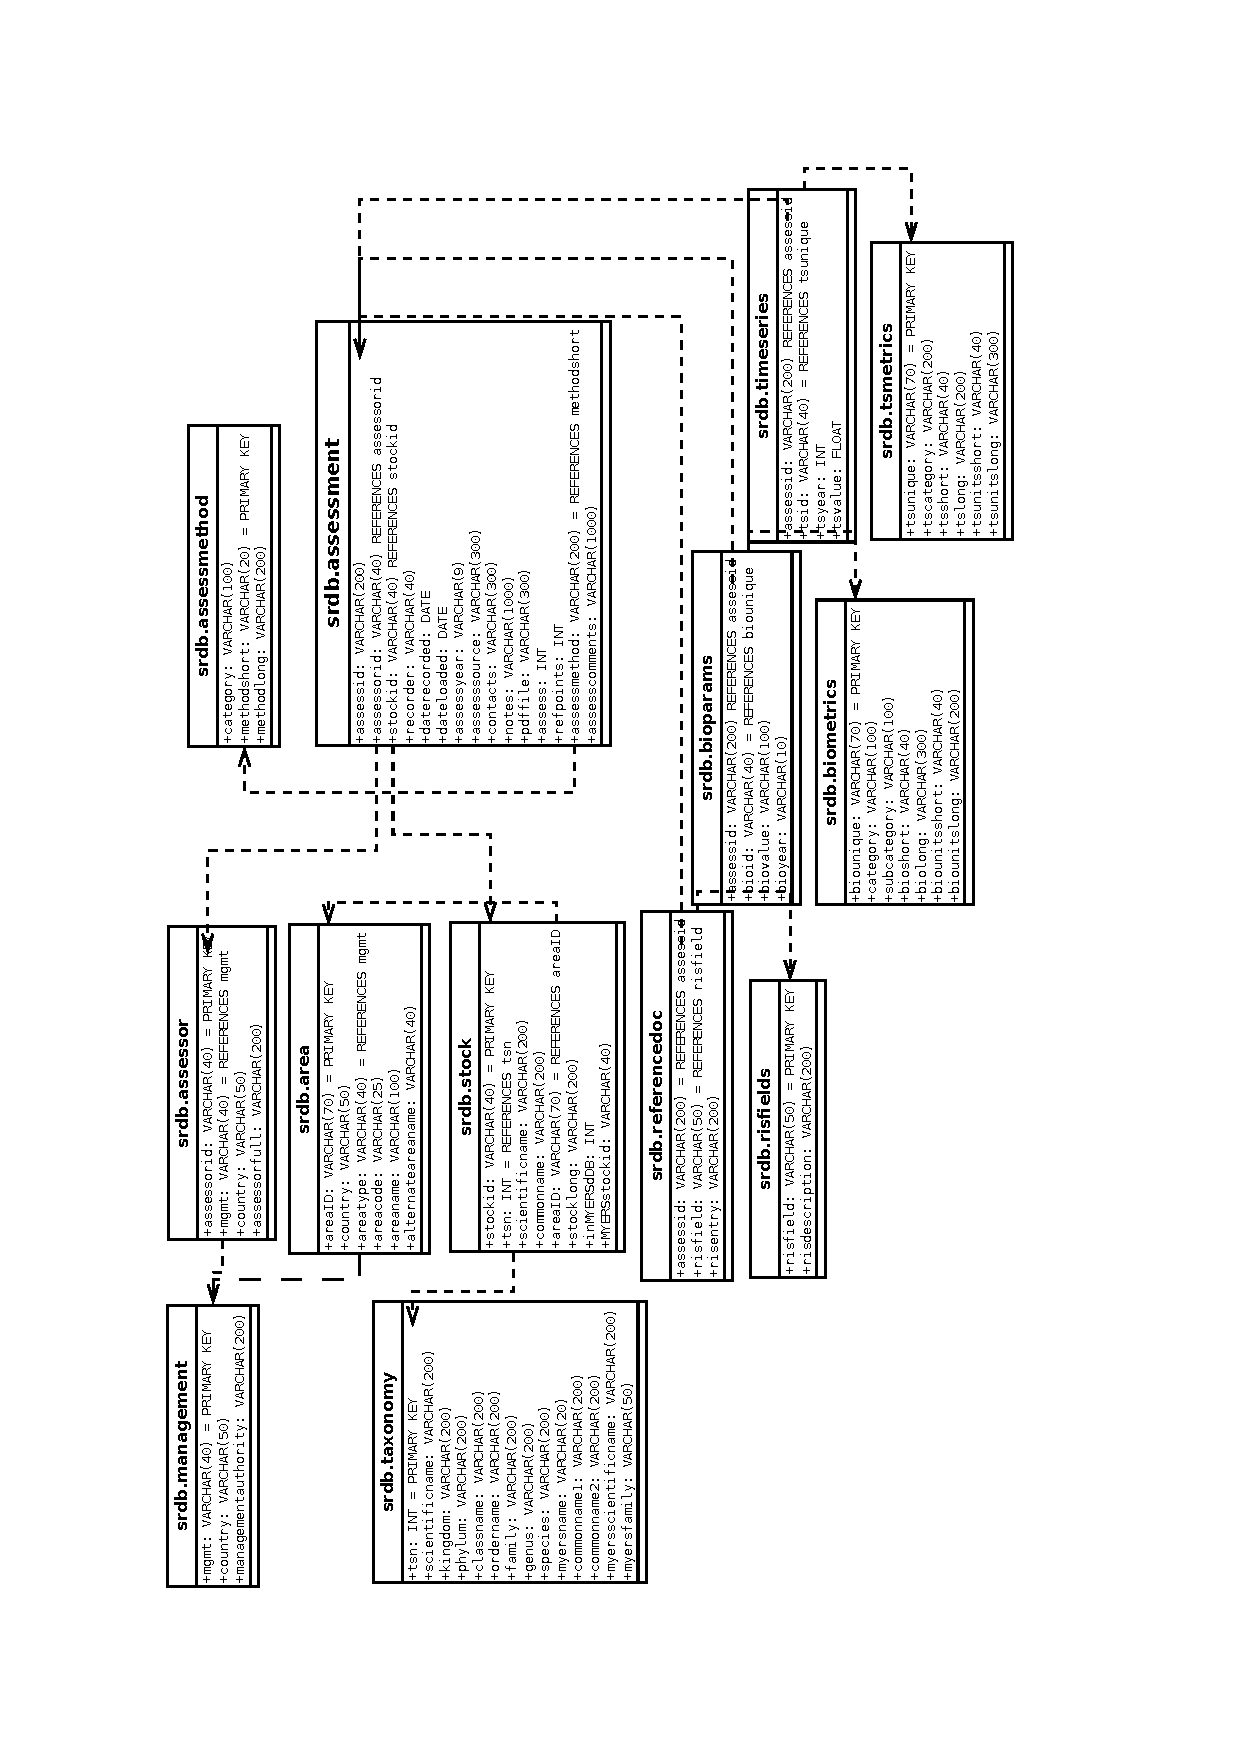
\includegraphics[width=15cm]{/home/srdbadmin/SQLpg/srdb/trunk/doc/srdb-ERD.pdf}
\end{center}
\caption{Entity relationship diagram of the RAM legacy database.}
\end{figure}


\begin{table}
\caption{Data used to generate Figure~\ref{fig:orca} - Summary of the assessments used in this analysis and the timespan of their different results. }
\begin{tabular}{| p{5cm} | p{3cm} | c | r  c  l | c | }\label{tab:timespan}
\textit{Fisheries stock} & \textit{Scientific name} & \textit{Timespan} & & \textit{Num. years available} & & \textit{Source} \\
 & & & Catch & SSB & R & \\
\hline \hline
blah & blah & 1970-2000 & 30 & 29 & 30 & (blah) \\
\end{tabular}
\end{table}


%\begin{table}
%\caption{Data used to generate Figures~\ref{fig:friedegg} and ~\ref{fig:friedeggmgmt} - Summary of the assessments used in this analysis and their estimated ratios of current biomass to the biomass at maximum sustainable yield and current harvest rate to the harvest rate that results is maximum sustainable yield. The estimated ratios were preferentially obtained directly from the assessment document or derived from surplus production model fits. When both an SSBmsy and Bmsy reference points are available, the SSB is chosen preferentially. }
%\begin{tabular}{| p{5cm} | p{3cm} | c | c | c | c | c |}\label{tab:crosshair}
%\textit{Fisheries stock} & \textit{Scientific name} & \textit{Current year} & \textit{B/Bmsy} & \textit{u/umsy} & \textit{From assessment?} & \textit{Source} \\
%\hline \hline
%blah & blah & 2000 & 1.0 & 1.0 & yes &  (blah) \\
%\end{tabular}
%\end{table}

% latex table generated in R 2.13.0 by xtable 1.5-6 package
% Thu May 19 14:38:14 2011
\begin{table}[ht]
\begin{center}
\begin{tabular}{ccc}
  \hline
 & SP U/Umsy $<$ 1 & SP U/Umsy $>$ 1 \\ 
  \hline
U/Umsy $<$ 1 &  20 &  14 \\ 
  U/Umsy $>$ 1 &   2 &   8 \\ 
  B/Bmsy $<$ 1 &  28 &   6 \\ 
  B/Bmsy $>$ 1 &  12 &  30 \\ 
   \hline
\end{tabular}
\caption{Contingency tables of stock status classification for biomass and exploitation reference points obtained from assessments and those derived from surplus production models. }
\label{tab:contingency}
\end{center}
\end{table}

\begin{table}[ht]
\begin{center}
\begin{tabular}{rllrrrl}
  \hline
 & stock & scientificname & currentyear & Bratio & Uratio & fromassessment \\
  \hline
1 & Alaska plaice Bering Sea and Aleutian Islands & Pleuronectes quadrituberculatus & 2008 & 2.46 & 0.05 & yes \\
  2 & Arrowtooth flounder Bering Sea and Aleutian Islands & Reinhardtius stomias & 2008 & 1.28 & 0.31 & no \\
  3 & Arrowtooth flounder Gulf of Alaska & Reinhardtius stomias & 2007 & 1.33 & 0.28 & no \\
  4 & Atka mackerel Bering Sea and Aleutian Islands & Pleurogrammus monopterygius & 2008 & 1.50 & 0.55 & no \\
  5 & Cabezon Northern California & Scorpaenichthys marmoratus & 2004 & 0.89 & 0.99 & no \\
  6 & Cabezon Southern California & Scorpaenichthys marmoratus & 2004 & 0.81 & 0.53 & no \\
  7 & Dusky rockfish Gulf of Alaska & Sebastes variabilis & 2007 & 1.54 & 0.54 & yes \\
  8 & Flathead sole Bering Sea and Aleutian Islands & Hippoglossoides elassodon & 2008 & 1.66 & 0.18 & no \\
  9 & Greenland turbot Bering Sea and Aleutian Islands & Reinhardtius hippoglossoides & 2009 & 1.48 & 0.05 & yes \\
  10 & Northern rockfish Bering Sea and Aleutian Islands & Sebastes polyspinis & 2008 & 1.07 & 0.13 & no \\
  11 & Northern rockfish Gulf of Alaska & Sebastes polyspinis & 2008 & 1.50 & 0.66 & yes \\
  12 & Northern rock sole Eastern Bering Sea and Aleutian Islands & Lepidopsetta polyxystra & 2007 & 3.02 & 0.21 & yes \\
  13 & Pacific cod Bering Sea and Aleutian Islands & Gadus macrocephalus & 2007 & 0.89 & 0.93 & no \\
  14 & Pacific cod Gulf of Alaska & Gadus macrocephalus & 2007 & 1.07 & 0.84 & no \\
  15 & Pacific Ocean perch Eastern Bering Sea and Aleutian Islands & Sebastes alutus & 2008 & 1.70 & 0.26 & no \\
  16 & Pacific ocean perch Gulf of Alaska & Sebastes alutus & 2008 & 1.16 & 0.73 & yes \\
  17 & Red king crab Bristol Bay & Paralithodes camtschaticus & 2007 & 0.00 & 1.38 & no \\
  18 & Sablefish Eastern Bering Sea / Aleutian Islands / Gulf of Alaska & Anoplopoma fimbria & 2008 & 0.72 & 0.90 & no \\
  19 & Snow crab Bering Sea & Chionoecetes opilio & 2008 & 0.29 & 1.61 & no \\
  20 & Walleye pollock Aleutian Islands & Theragra chalcogramma & 2008 & 0.86 & 0.02 & yes \\
  21 & Walleye pollock Eastern Bering Sea & Theragra chalcogramma & 2008 & 0.68 & 0.85 & no \\
  22 & Yellowfin sole Bering Sea and Aleutian Islands & Limanda aspera & 2008 & 1.94 & 0.62 & yes \\
  23 & Capelin Barents Sea & Mallotus villosus & 2006 & 0.17 & 0.00 & no \\
  24 & Atlantic cod coastal Norway & Gadus morhua & 2006 & 0.20 & 2.57 & no \\
  25 & Atlantic cod Northeast Arctic & Gadus morhua & 2006 & 0.56 & 1.42 & no \\
  26 & Greenland halibut Northeast Arctic & Reinhardtius hippoglossoides & 2006 & 0.23 & 1.38 & no \\
  27 & Golden Redfish Northeast Arctic & Sebastes norvegicus & 2006 & 0.00 & 4.25 & no \\
  28 & Haddock Northeast Arctic & Melanogrammus aeglefinus & 2006 & 1.10 & 1.06 & no \\
  29 & Pollock Northeast Arctic & Pollachius virens & 2006 & 1.70 & 0.60 & no \\
  30 & Atlantic croaker Mid-Atlantic Coast & Micropogonias undulatus & 2002 & 1.42 & 0.27 & yes \\
  31 & Northern shrimp Gulf of Maine & Pandalus borealis & 2008 & 1.58 & 0.56 & no \\
  32 & Antarctic toothfish Ross Sea & Dissostichus mawsoni & 2007 & 1.76 & 1.09 & no \\
  33 & Deepwater flathead Southeast Australia & Platycephalus conatus & 2006 & 1.33 & 0.61 & no \\
  34 & common gemfish Southeast Australia & Rexea solandri & 2007 & 0.01 & 0.59 & no \\
  35 & Jackass morwong Southeast Australia & Nemadactylus macropterus & 2007 & 0.25 & 1.80 & no \\
  36 & New Zealand ling Eastern half of Southeast Australia & Genypterus blacodes & 2007 & 0.60 & 2.20 & no \\
  37 & Orange roughy Cascade Plateau & Hoplostethus atlanticus & 2006 & 1.76 & 0.34 & no \\
  38 & Orange roughy Southeast Australia & Hoplostethus atlanticus & 2006 & 0.89 & 0.29 & no \\
  39 & Silverfish Southeast Australia & Seriolella punctata & 2006 & 1.15 & 0.79 & no \\
  40 & School whiting Southeast Australia & Sillago flindersi & 2007 & 1.10 & 0.82 & no \\
  41 & Tiger flathead Southeast Australia & Neoplatycephalus richardsoni & 2006 & 1.05 & 0.00 & no \\
  42 & Blue Warehou Eastern half of Southeast Australia & Seriolella brama & 2006 & 0.17 & 0.84 & no \\
  43 & Blue Warehou Western half of Southeast Australia & Seriolella brama & 2006 & 0.62 & 2.04 & no \\
  44 & Atlantic cod NAFO 5Zjm & Gadus morhua & 2002 & 0.00 & 0.74 & no \\
  45 & Haddock NAFO-4X5Y & Melanogrammus aeglefinus & 2003 & 0.28 & 0.45 & no \\
  46 & Haddock NAFO-5Zejm & Melanogrammus aeglefinus & 2002 & 0.15 & 0.86 & no \\
  47 & Atlantic cod NAFO 2J3KL inshore & Gadus morhua & 2005 & 1.60 & 0.14 & no \\
  48 & Atlantic cod NAFO 3Ps & Gadus morhua & 2004 & 0.43 & 0.43 & no \\
  49 & English sole Hecate Strait & Parophrys vetulus & 2001 & 1.23 & 0.37 & no \\
  50 & Pacific herring Central Coast & Clupea pallasii & 2007 & 0.30 & 0.11 & no \\
  51 & Pacific herring Prince Rupert District & Clupea pallasii & 2007 & 0.00 & 0.44 & no \\
  52 & Pacific herring Queen Charlotte Islands & Clupea pallasii & 2007 & 0.20 & 0.00 & no \\
  53 & Pacific herring Straight of Georgia & Clupea pallasii & 2007 & 0.91 & 0.40 & no \\
  54 & Pacific herring West Coast of Vancouver Island & Clupea pallasii & 2007 & 0.03 & 0.00 & no \\
  55 & Pacific cod Hecate Strait & Gadus macrocephalus & 2004 & 0.37 & 0.25 & no \\
  56 & Pacific cod West Coast of Vancouver Island & Gadus macrocephalus & 2001 & 0.28 & 0.61 & no \\
  57 & Rock sole Hecate Strait & Lepidopsetta bilineata & 2001 & 1.03 & 0.45 & no \\
  58 & Pollock NAFO-4VWX5Zc & Pollachius virens & 2006 & 0.56 & 0.30 & no \\
  59 & Atlantic cod NAFO 3Pn4RS & Gadus morhua & 2006 & 0.03 & 1.09 & no \\
  60 & Atlantic cod NAFO 4TVn & Gadus morhua & 2006 & 0.17 & 0.32 & no \\
  61 & Herring ICES 22-24-IIIa & Clupea harengus & 2006 & 0.73 & 1.02 & no \\
  62 & Herring Northern Irish Sea & Clupea harengus & 2006 & 0.72 & 0.34 & no \\
  63 & Herring North Sea & Clupea harengus & 2006 & 0.65 & 1.32 & no \\
  64 & Herring ICES VIa & Clupea harengus & 2006 & 0.18 & 1.59 & no \\
  65 & Herring ICES VIa-VIIb-VIIc & Clupea harengus & 2000 & 0.50 & 1.04 & no \\
  66 & Albacore tuna North Atlantic & Thunnus alalunga & 2005 & 0.81 & 1.49 & yes \\
  67 & Bluefin tuna Eastern Atlantic & Thunnus thynnus & 2007 & 0.34 & 9.38 & yes \\
  68 & Bluefin tuna Western Atlantic & Thunnus thynnus & 2007 & 0.57 & 1.33 & yes \\
  69 & Bigeye tuna Atlantic & Thunnus obesus & 2005 & 0.90 & 0.86 & no \\
  70 & Skipjack tuna Eastern Atlantic & Katsuwonus pelamis & 2006 & 1.71 & 0.27 & no \\
  71 & Skipjack tuna Western Atlantic & Katsuwonus pelamis & 2006 & 1.72 & 0.27 & no \\
  72 & Swordfish Mediterranean Sea & Xiphias gladius & 2006 & 0.94 & 1.27 & yes \\
  73 & Swordfish North Atlantic & Xiphias gladius & 2005 & 1.03 & 0.82 & no \\
  74 & Swordfish South Atlantic & Xiphias gladius & 2005 & 1.18 & 0.69 & no \\
  75 & Yellowfin tuna Atlantic & Thunnus albacares & 2006 & 1.07 & 0.81 & yes \\
  76 & Chilean jack mackerel Chilean EEZ and offshore & Trachurus murphyi & 2006 & 0.52 & 1.20 & no \\
  77 & Argentine anchoita Northern Argentina & Engraulis anchoita & 2007 & 1.37 & 0.17 & yes \\
  78 & Argentine anchoita Southern Argentina & Engraulis anchoita & 2007 & 3.13 & 0.04 & yes \\
  79 & Argentine hake Northern Argentina & Merluccius hubbsi & 2007 & 0.16 & 1.26 & yes \\
  80 & Argentine hake Southern Argentina & Merluccius hubbsi & 2008 & 0.34 & 1.49 & yes \\
  81 & Patagonian grenadier Southern Argentina & Macruronus magellanicus & 2006 & 1.82 & 0.60 & yes \\
  82 & Bigeye tuna Indian Ocean & Thunnus obesus & 2004 & 1.23 & 0.97 & yes \\
  83 & Pacific halibut North Pacific & Hippoglossus stenolepis & 2008 & 0.54 & 2.01 & no \\
  84 & Anchovy South Africa & Engraulis encrasicolus & 2006 & 0.97 & 0.36 & no \\
  85 & Shallow-water cape hake South Africa & Merluccius capensis & 2008 & 1.16 & 0.40 & no \\
  86 & Cape horse mackerel South Africa South coast & Trachurus capensis & 2007 & 1.47 & 0.76 & no \\
  87 & Kingklip South Africa & Engraulis encrasicolus & 2008 & 1.13 & 0.55 & no \\
  88 & Sardine South Africa & Sardinops sagax & 2006 & 0.75 & 0.55 & no \\
  89 & Southern spiny lobster South Africa South coast & Palinurus gilchristi & 2008 & 0.51 & 1.50 & no \\
  90 & American Plaice NAFO-3LNO & Hippoglossoides platessoides & 2006 & 0.02 & 1.05 & no \\
  91 & American Plaice NAFO-3M & Hippoglossoides platessoides & 2007 & 0.00 & 0.00 & no \\
  92 & Atlantic cod NAFO 3NO & Gadus morhua & 2006 & 0.00 & 0.38 & no \\
  93 & Greenland halibut NAFO 23KLMNO & Reinhardtius hippoglossoides & 2006 & 0.39 & 1.73 & no \\
  94 & Redfish species NAFO 3LN & Redfish species & 2008 & 1.88 & 0.04 & yes \\
  95 & Redfish species NAFO 3M & Redfish species & 2006 & 0.93 & 0.15 & no \\
  96 & Yellowtail Flounder NAFO 3LNO & Limanda ferruginea & 2007 & 1.62 & 0.15 & no \\
  97 & American Plaice NAFO-5YZ & Hippoglossoides platessoides & 2007 & 0.55 & 0.30 & no \\
  98 & Bluefish Atlantic Coast & Pomatomus saltatrix & 2007 & 0.81 & 1.25 & no \\
  99 & Black sea bass Mid-Atlantic Coast & Centropristis striata & 2007 & 1.21 & 0.67 & no \\
  100 & Atlantic cod Georges Bank & Gadus morhua & 2007 & 0.00 & 1.15 & no \\
  101 & Atlantic cod Gulf of Maine & Gadus morhua & 2007 & 1.46 & 0.29 & no \\
  102 & Haddock NAFO-5Y & Melanogrammus aeglefinus & 2007 & 0.00 & 1.86 & no \\
  103 & Monkfish Gulf of Maine / Northern Georges Bank & Lophius americanus & 2006 & 1.73 & 0.38 & no \\
  104 & Monkfish Southern Georges Bank / Mid-Atlantic & Lophius americanus & 2006 & 1.72 & 0.30 & no \\
  105 & Sea scallop Georges Bank & Placopecten magellanicus & 2006 & 1.59 & 0.78 & no \\
  106 & Sea scallop Mid-Atlantic Coast & Placopecten magellanicus & 2006 & 0.91 & 0.37 & no \\
  107 & Spiny dogfish Atlantic Coast & Squalus acanthias & 2005 & 1.61 & 0.15 & no \\
  108 & Atlantic surfclam Mid-Atlantic Coast & Spisula solidissima & 1994 & 1.85 & 0.00 & no \\
  109 & Tilefish Mid-Atlantic Coast & Lopholatilus chamaeleonticeps & 2005 & 0.72 & 0.61 & no \\
  110 & Weakfish Atlantic Coast & Cynoscion regalis & 2008 & 0.06 & 1.49 & no \\
  111 & White hake Georges Bank / Gulf of Maine & Urophycis tenuis & 2007 & 0.35 & 0.80 & yes \\
  112 & Winter Flounder NAFO-5Z & Pseudopleuronectes americanus & 2006 & 1.41 & 0.25 & no \\
  113 & Winter Flounder Southern New England-Mid Atlantic & Pseudopleuronectes americanus & 2007 & 0.07 & 1.44 & no \\
  114 & Witch Flounder NAFO-5Y & Glyptocephalus cynoglossus & 2007 & 0.30 & 1.45 & yes \\
  115 & Yellowtail flounder Cape Cod / Gulf of Maine & Limanda ferruginea & 2007 & 0.25 & 1.73 & yes \\
  116 & Yellowtail flounder Georges Bank & Limanda ferruginea & 2007 & 0.22 & 1.14 & yes \\
  117 & Yellowtail Flounder Southern New England-Mid Atlantic & Limanda ferruginea & 2007 & 0.13 & 1.61 & yes \\
  118 & Australian salmon New Zealand & Arripis trutta & 2006 & 1.64 & 0.33 & yes \\
  119 & Orange roughy New Zealand Mid East Coast & Hoplostethus atlanticus & 2004 & 1.20 & 0.35 & yes \\
  120 & Atlantic menhaden Atlantic & Brevoortia tyrannus & 2005 & 0.47 & 0.97 & no \\
  121 & Pacific sardine North Pacific & Sardinops sagax & 2006 & 1.73 & 0.37 & no \\
  122 & Arrowtooth flounder Pacific Coast & Reinhardtius stomias & 2007 & 3.81 & 0.21 & yes \\
  123 & Blackgill rockfish  Pacific Coast & Sebastes melanostomus & 2004 & 0.80 & 1.20 & no \\
  124 & Black rockfish Northern Pacific Coast & Sebastes melanops & 2006 & 1.37 & 0.57 & no \\
  125 & Black rockfish Southern Pacific Coast & Sebastes melanops & 2007 & 2.23 & 0.33 & yes \\
  126 & Blue rockfish California & Sebastes mystinus & 2007 & 0.75 & 1.19 & yes \\
  127 & Bocaccio Southern Pacific Coast & Sebastes paucispinis & 2006 & 0.32 & 0.10 & yes \\
  128 & Chilipepper Southern Pacific Coast & Sebastes goodei & 2006 & 1.43 & 0.04 & no \\
  129 & Cowcod Southern California & Sebastes levis & 2007 & 0.09 & 0.07 & yes \\
  130 & Canary rockfish Pacific Coast & Sebastes pinniger & 2007 & 0.85 & 0.02 & yes \\
  131 & Darkblotched rockfish Pacific Coast & Sebastes crameri & 2007 & 0.73 & 0.31 & yes \\
  132 & English sole Pacific Coast & Parophrys vetulus & 2006 & 2.06 & 0.14 & no \\
  133 & Longnose skate Pacific Coast & Raja rhina & 2007 & 1.56 & 0.40 & no \\
  134 & Longspine thornyhead Pacific Coast & Sebastolobus altivelis & 2005 & 2.65 & 0.23 & yes \\
  135 & Pacific hake Pacific Coast & Merluccius productus & 2007 & 0.42 & 1.67 & no \\
  136 & Pacific ocean perch Pacific Coast & Sebastes alutus & 2007 & 0.69 & 0.00 & yes \\
  137 & Petrale sole Northern Pacific Coast & Eopsetta jordani & 2004 & 0.96 & 1.26 & no \\
  138 & Petrale sole Southern Pacific Coast & Eopsetta jordani & 2004 & 0.63 & 0.61 & no \\
  139 & Sablefish Pacific Coast & Anoplopoma fimbria & 2007 & 0.84 & 1.09 & no \\
  140 & Shortspine thornyhead Pacific Coast & Sebastolobus alascanus & 2004 & 1.55 & 0.93 & no \\
  141 & Widow rockfish Pacific Coast & Sebastes entomelas & 2006 & 0.91 & 0.07 & no \\
  142 & Yelloweye rockfish Pacific Coast & Sebastes ruberrimus & 2006 & 0.38 & 0.34 & no \\
  143 & Yellowtail rockfish Northern Pacific Coast & Sebastes flavidus & 2005 & 0.75 & 0.51 & no \\
  144 & Capelin Iceland & Mallotus villosus & 2006 & 0.49 & 0.85 & no \\
  145 & Atlantic cod Faroe Plateau & Gadus morhua & 2006 & 0.26 & 1.52 & no \\
  146 & Atlantic cod Iceland & Gadus morhua & 2006 & 0.46 & 1.17 & no \\
  147 & Haddock Faroe Plateau & Melanogrammus aeglefinus & 2006 & 0.85 & 1.07 & no \\
  148 & Haddock Iceland & Melanogrammus aeglefinus & 2007 & 0.73 & 1.36 & no \\
  149 & Pollock Faroe Plateau & Pollachius virens & 2006 & 0.99 & 1.52 & no \\
  150 & Black oreo West end of Chatham Rise & Allocyttus niger & 2007 & 0.99 & 0.82 & yes \\
  151 & Smooth oreo Chatham Rise & Pseudocyttus maculatus & 2006 & 2.25 & 0.38 & yes \\
  152 & Smooth oreo West end of Chatham Rise & Pseudocyttus maculatus & 2004 & 1.25 & 0.53 & yes \\
  153 & Hoki Eastern New Zealand & Macruronus novaezelandiae & 2007 & 1.11 & 0.33 & no \\
  154 & Hoki Western New Zealand & Macruronus novaezelandiae & 2007 & 0.51 & 0.57 & no \\
  155 & New Zealand snapper New Zealand Area 8 & Chrysophrys auratus & 2005 & 0.35 & 2.50 & yes \\
  156 & Trevally New Zealand Areas TRE 7 & Pseudocaranx dentex & 2005 & 1.44 & 0.83 & yes \\
  157 & Red rock lobster New Zealand area CRA1 & Jasus edwardsii & 2001 & 1.14 & 0.88 & no \\
  158 & Red rock lobster New Zealand area CRA2 & Jasus edwardsii & 2001 & 0.53 & 2.12 & no \\
  159 & Red rock lobster New Zealand area CRA4 & Jasus edwardsii & 2005 & 0.67 & 1.33 & no \\
  160 & Red rock lobster New Zealand area CRA5 & Jasus edwardsii & 2002 & 0.59 & 1.68 & no \\
  161 & Red rock lobster New Zealand area CRA7 & Jasus edwardsii & 2005 & 0.73 & 0.43 & no \\
  162 & Red rock lobster New Zealand area CRA8 & Jasus edwardsii & 2005 & 0.69 & 0.49 & no \\
  163 & common gemfish New Zealand & Rexea solandri & 2006 & 1.64 & 0.43 & yes \\
  164 & New Zealand ling New Zealand Areas LIN 3 and 4 & Genypterus blacodes & 2007 & 3.07 & 0.09 & yes \\
  165 & New Zealand ling New Zealand Areas LIN 5 and 6 & Genypterus blacodes & 2007 & 3.96 & 0.10 & yes \\
  166 & New Zealand ling New Zealand Area LIN 6b & Genypterus blacodes & 2006 & 2.19 & 0.11 & yes \\
  167 & New Zealand ling New Zealand Area LIN 72 & Genypterus blacodes & 2007 & 2.49 & 0.32 & yes \\
  168 & New Zealand ling New Zealand Area LIN 7WC - WCSI & Genypterus blacodes & 2008 & 2.21 & 0.13 & yes \\
  169 & Southern blue whiting Campbell Island Rise & Micromesistius australis & 2006 & 1.15 & 0.92 & yes \\
  170 & Southern hake Chatham Rise & Merluccius australis & 2006 & 1.77 & 0.12 & yes \\
  171 & Southern hake Sub-Antarctic & Merluccius australis & 2007 & 2.91 & 0.11 & yes \\
  172 & New Zealand abalone species New Zealand Area PAU 5A & Haliotis iris & 2006 & 0.72 & 2.83 & no \\
  173 & New Zealand abalone species New Zealand Area PAU 5B & Haliotis iris & 2007 & 1.02 & 0.59 & no \\
  174 & New Zealand abalone species New Zealand Area PAU 5D & Haliotis iris & 2006 & 0.44 & 2.10 & no \\
  175 & New Zealand abalone species New Zealand Area PAU 7 & Haliotis iris & 2008 & 0.87 & 0.94 & no \\
  176 & American lobster Rhode Island & Homarus americanus & 2006 & 0.51 & 0.68 & no \\
  177 & Tautog Rhode Island & Tautoga onitis & 2006 & 0.84 & 0.59 & no \\
  178 & Winter flounder Rhode Island & Pseudopleuronectes americanus & 2006 & 0.03 & 2.35 & no \\
  179 & Gag Gulf of Mexico & Mycteroperca microlepis & 2004 & 1.25 & 1.84 & no \\
  180 & Gag Southern Atlantic coast & Mycteroperca microlepis & 2005 & 0.94 & 1.31 & yes \\
  181 & Greater amberjack Gulf of Mexico & Seriola dumerili & 2004 & 0.46 & 1.52 & no \\
  182 & King mackerel Gulf of Mexico & Scomberomorus cavalla & 2001 & 1.51 & 0.44 & no \\
  183 & King mackerel Southern Atlantic Coast & Scomberomorus cavalla & 2001 & 1.38 & 0.56 & no \\
  184 & Gulf menhaden Gulf of Mexico & Brevoortia patronus & 2004 & 1.08 & 0.48 & no \\
  185 & Red grouper Gulf of Mexico & Epinephelus morio & 2005 & 0.17 & 1.39 & no \\
  186 & Red porgy Southern Atlantic coast & Pagrus pagrus & 2004 & 0.61 & 0.39 & yes \\
  187 & Snowy grouper Southern Atlantic coast & Epinephelus niveatus & 2002 & 0.19 & 3.08 & yes \\
  188 & Spanish mackerel Southern Atlantic Coast & Scomberomorus maculatus & 2007 & 0.38 & 0.91 & yes \\
  189 & Tilefish Southern Atlantic coast & Lopholatilus chamaeleonticeps & 2002 & 0.94 & 1.55 & yes \\
  190 & Vermilion snapper Southern Atlantic coast & Rhomboplites aurorubens & 2007 & 0.86 & 1.27 & yes \\
  191 & Yellowtail snapper Southern Atlantic Coast and Gulf of Mexico & Ocyurus chrysurus & 2001 & 1.14 & 0.61 & yes \\
  192 & Walleye pollock Northern Sea of Okhotsk & Theragra chalcogramma & 1992 & 1.11 & 0.87 & no \\
  193 & Albacore tuna South Pacific Ocean & Thunnus alalunga & 2006 & 2.46 & 0.90 & yes \\
  194 & Bigeye tuna Western Pacific Ocean & Thunnus obesus & 2006 & 1.06 & 1.38 & yes \\
  195 & Skipjack tuna Central Western Pacific & Katsuwonus pelamis & 2006 & 4.38 & 0.30 & yes \\
  196 & Yellowfin tuna Central Western Pacific & Thunnus albacares & 2005 & 1.22 & 0.80 & yes \\
  197 & Dover sole Pacific Coast & Microstomus pacificus & 2004 & 1.33 & 0.45 & no \\
  198 & Gopher rockfish Southern Pacific Coast & Sebastes carnatus & 2004 & 1.69 & 0.08 & no \\
  199 & Pacific sardine Pacific Coast & Sardinops sagax & 2006 & 1.36 & 0.41 & no \\
  200 & Starry flounder Northern Pacific Coast & Platichthys stellatus & 2004 & 0.68 & 0.33 & no \\
  201 & Starry flounder Southern Pacific Coast & Platichthys stellatus & 2004 & 1.15 & 0.12 & no \\
  202 & Tasmanian giant crab Tasmania & Pseudocarcinus gigas & 2007 & 0.50 & 1.71 & no \\
  203 & Walleye pollock Western Bering Sea & Theragra chalcogramma & 2004 & 2.16 & 0.26 & no \\
  204 & Atlantic cod Baltic Areas 22 and 24 & Gadus morhua & 2006 & 0.31 & 1.55 & no \\
  205 & Atlantic cod Baltic Areas 25-32 & Gadus morhua & 2006 & 0.14 & 1.58 & no \\
  206 & Atlantic cod Kattegat & Gadus morhua & 2006 & 0.19 & 0.31 & no \\
  207 & Herring ICES 25-32 & Clupea harengus & 2006 & 0.69 & 0.79 & no \\
  208 & Herring ICES 30 & Clupea harengus & 2006 & 1.19 & 1.10 & no \\
  209 & Herring ICES 31 & Clupea harengus & 2006 & 0.27 & 1.65 & no \\
  210 & Herring Iceland (Summer spawners) & Clupea harengus & 2006 & 0.70 & 0.89 & no \\
  211 & Herring ICES 28 & Clupea harengus & 2006 & 1.21 & 0.87 & no \\
  212 & common European sole ICES Kattegat and Skagerrak & Solea vulgaris & 2006 & 1.25 & 0.54 & no \\
  213 & Sprat ICES Baltic Areas 22-32 & Sprattus sprattus & 2006 & 1.13 & 1.27 & no \\
  214 & Fourspotted megrim ICES VIIIc-IXa & Lepidorhombus boscii & 2006 & 0.00 & 1.61 & no \\
  215 & Hake Northeast Atlantic North & Merluccius merluccius & 2006 & 1.04 & 0.74 & no \\
  216 & Megrim ICES VIIIc-IXa & Lepidorhombus whiffiagonis & 2006 & 0.24 & 1.31 & no \\
  217 & common European sole Bay of Biscay & Solea vulgaris & 2006 & 0.62 & 1.13 & no \\
  218 & Mackerel ICES Northeast Atlantic & Scomber scombrus & 2006 & 0.98 & 0.73 & no \\
  219 & Whiting Northeast Atlantic & Micromesistius poutassou & 2006 & 0.67 & 1.66 & no \\
  220 & Atlantic cod Irish Sea & Gadus morhua & 2006 & 0.09 & 0.69 & no \\
  221 & Atlantic cod West of Scotland & Gadus morhua & 2006 & 0.10 & 0.45 & no \\
  222 & Haddock West of Scotland & Melanogrammus aeglefinus & 2006 & 0.58 & 0.73 & no \\
  223 & European Plaice Irish Sea & Pleuronectes platessa & 2006 & 1.07 & 0.23 & no \\
  224 & common European sole Irish Sea & Solea vulgaris & 2006 & 0.36 & 1.16 & no \\
  225 & Atlantic cod North Sea & Gadus morhua & 2006 & 0.19 & 0.80 & no \\
  226 & Haddock ICES IIIa and North Sea & Melanogrammus aeglefinus & 2006 & 0.62 & 0.25 & no \\
  227 & Haddock Rockall Bank & Melanogrammus aeglefinus & 2006 & 1.10 & 0.52 & no \\
  228 & Norway pout North Sea & Trisopterus esmarkii & 2006 & 0.90 & 0.33 & no \\
  229 & Pollock ICES IIIa, VI and North Sea & Pollachius virens & 2006 & 0.56 & 0.97 & no \\
  230 & Sandeel North Sea & Ammodytes marinus & 2007 & 0.92 & 0.24 & no \\
  231 & Whiting ICES IIIa, VIId and North Sea & Merlangius merlangus & 2006 & 0.33 & 1.04 & no \\
  232 & Haddock ICES VIIb-k & Melanogrammus aeglefinus & 2006 & 1.37 & 0.41 & no \\
  233 & European Plaice ICES VIIf-g & Pleuronectes platessa & 2006 & 0.65 & 0.41 & no \\
  234 & European Plaice ICES VIIe & Pleuronectes platessa & 2006 & 0.51 & 1.39 & no \\
  235 & common European sole Celtic Sea & Solea vulgaris & 2006 & 0.90 & 0.95 & no \\
  236 & common European sole Western English Channel & Solea vulgaris & 2006 & 0.51 & 1.75 & no \\
  237 & Whiting ICES VIIe-k & Merlangius merlangus & 2006 & 0.44 & 1.25 & no \\
   \hline
\end{tabular}
\caption{Data used to generate Figures~\ref{fig:friedegg} and ~\ref{fig:friedeggmgmt} - Summary of the assessments used in this analysis and their estimated ratios of current biomass to the biomass at maximum sustainable yield and current harvest rate to the harvest rate that results is maximum sustainable yield. The estimated ratios were preferentially obtained directly from the assessment document or derived from surplus production model fits. When both an SSBmsy and Bmsy reference points are available, the SSB is chosen preferentially.}
\label{tab:crosshair}
\end{center}
\end{table}

\end{document}
